\doublespacing
\chapter{Experimentos}\label{sec:experiments}
\doublespacing
%======================================================================================
Os experimentos se concentram em explorar, ao longo deste Capítulo, os objetivos citados anteriormente, no início deste documento.

\section{Procedimento}
Primeiramente, foram realizadas filmagens iniciais de algumas esculturas,
utilizando-se a câmera de um \emph{smartphone} convencional, primariamente um
iPhone 5s, na resolução \emph{Full HD} de 1920x1080 pixels. Esta filmagem foi realizada de
forma conveniente a um usuário leigo, sem grandes restrições, procurando-se
varrer a maioria da superfície da escultura em $360^{\circ}$,
Figura~\ref{fig:procedimentoscan}.  Em seguida, fizemos mais alguns vídeos,
capturando alguns pontos que possuíam mais detalhes mais de perto.

Vale ressaltar que no dia das filmagens, estava ensolarado com boa iluminação para a captura das esculturas.

\begin{figure}[!h]
	\centering
\caption{%
	Como foi realizada a varredura das esculturas
	}	
	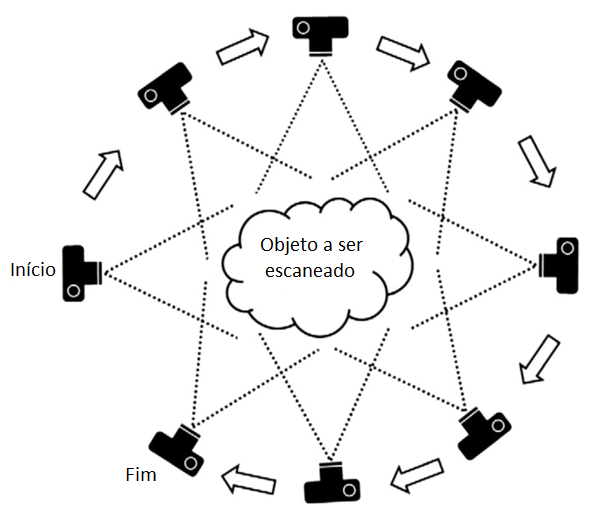
\includegraphics[width=0.4\linewidth]{figs/procedimentoscan.png}
	\source{
   	 O autor,
   	 2017.
   }\label{fig:procedimentoscan}
\end{figure}

Com este material, foram feitos videoclipes extraindo um subconjunto de
\emph{frames} do vídeo, para ao menos inicialmente não utilizarmos uma quantidade muito
grande de imagens. Houve atenção para não extrair apenas \emph{frames} muito
juntos, pois aumentaria o número de correspondências ambíguas entre as imagens e
com isso, o processamento da reconstrução demoraria mais. Também procurou-se 
evitar usar apenas \emph{frames} muito distantes, pulando os muito próximos,
pois ocorreria o inverso: com menos
correspondências, ficariam buracos (partes sem a informação necessária) na
reconstrução, como descrito na Seção~\ref{sec:mve}.
Com isso em mente, nos experimentos iniciais foram reconstruídas duas esculturas
empregando o VisualSfM, totalizando 197 imagens, 
%
%guerreiro, indio% 
%
e, com o MVE, utilizamos dois vídeos, que, ao selectionar os frames, totalizou cerca de 280
imagens.
Para critério de comparação, usamos o tempo de reconstrução nos dois programas que é importante para termos um parâmetro de quanto demoraria para reconstruirmos uma escultura com mais, ou com menos imagens. E também as áreas faltantes nas reconstruções, avaliando a qualidade da reconstrução e o nível de detalhes obtidos com os softwares.
%
%sapo%

Além de esculturas ao ar livre, fizemos alguns testes em ambiente fechado,
dentro de uma casa, por exemplo. Foi utilizado um objeto feito de cabaça (casca
de abóbora), a qual possui uma reflectância propícia
(Lambertiana) para uma reconstrução~\cite{basri2003lambertian}, ao mesmo tempo
sendo um objeto de arte e suave, com certos desafios similares às esculturas do
Jardim do Nêgo.  Com o procedimento descrito anteriormente, a partir dos vídeos
feitos, selecionamos um total de 200 imagens em um vídeo superficial e mais 24
imagens mais detalhadas do objeto, ambos numa resolução de 1080x1920 pixels. 
Para um mesmo conjunto de imagens, foi executado tanto o VisualSfM quanto o MVE.
%KINECT
%Para um mesmo conjunto de imagens, foi executado o VisualSfM, o MVE e o Skanect versão gratuita do Kinect.


\subsection{Resultados da reconstrução com o VisualSfM}

Seguindo o passo-a-passo de reconstrução do software, obtivemos os seguintes
resultados em relação ao tempo, Tabela~\ref{tab:temposSfMJardimDoNego}. Para a escultura de
197 imagens do Jardim do Nêgo, com as reconstruções mostradas nas
Figuras~\ref{fig:reconstrucaoEsparsaIndioVisualSFM} e~\ref{fig:reconstrucaoDensaIndioVisualSFM}.

\newpage

\begin{table}[h!]
\caption{Tempos obtidos da reconstrução da escultura do Jardim do Nêgo usando o VisualSfM}
\label{tab:temposSfMJardimDoNego}
\begin{tabular}{|l|p{4.7cm}|}
\hline
Procedimento & Tempo (aprox.) \\ \hline
Carregamento de imagens & 10 segundos \\ \hline
Calcular pares correspondentes de \emph{features} & 1 hora e 50 minutos \\ \hline
Gerar a reconstrução esparsa do modelo & 4 minutos \\ \hline
Gerar a reconstrução densa do modelo & 24 minutos \\ \hline
\end{tabular}
	\source{
   	 O autor,
   	 2017.
   }
\end{table}

Percebe-se que foi gerada uma nuvem de pontos bastante consistente, a partir da
reconstrução esparsa do algoritmo PBA.  Por conta disso, nossa reconstrução 3D
densa, empregando o MCBA/PMVS-2, obteve uma qualidade razoável para o conjunto de
imagens usado, apesar de apresentar ainda ruídos e falta de resolução para uma
preservação de patrimônio completa como no projeto \emph{Digital Michaelangelo}
de escaneamento a laser. Nota-se que o resultado é bastante surpreendente, dado que
apenas os vídeos foram fornecidos, e o software teve que calcular as posições
das câmeras, além da e reconstrução geométrica e fotométrica.
%COLOCAR IMAGENS GUERREIRO AQUI%

\begin{figure}[!h]
	\centering
	\caption{%
	Reconstrução esparsa da escultura do Jardim do Nêgo no VisualSfM com 197 imagens.
	}
	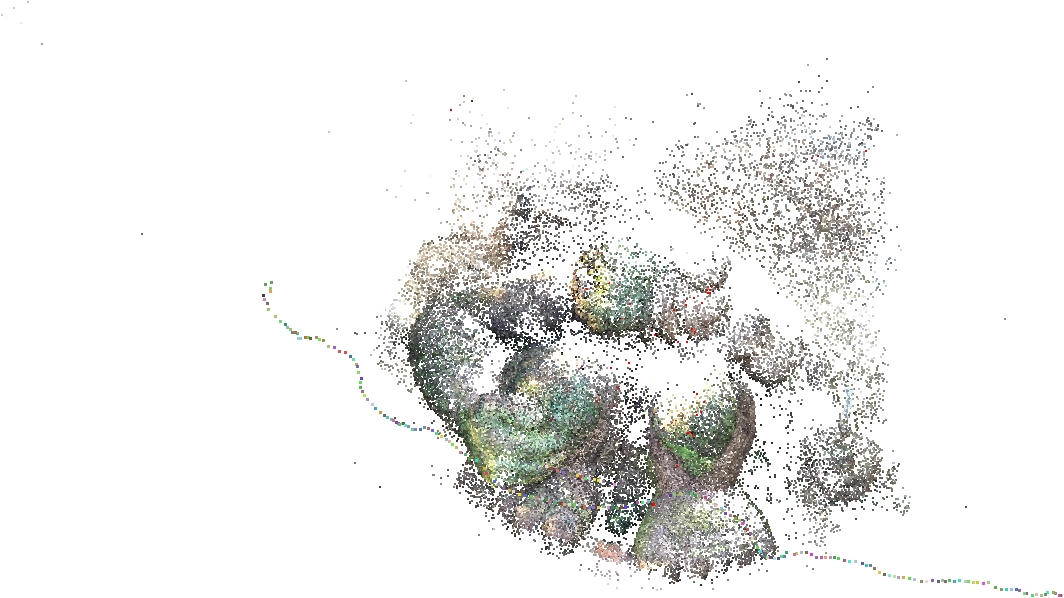
\includegraphics[width=0.9\linewidth]{figs/guerreiroEsparsa.jpg}
		\source{
   	 O autor,
   	 2017.
   }\label{fig:reconstrucaoEsparsaIndioVisualSFM}
\end{figure}

\newpage

\begin{figure}[!h]
	\centering
	\caption{Resultados da reconstrução densa da escultura do Jardim do Nêgo}
	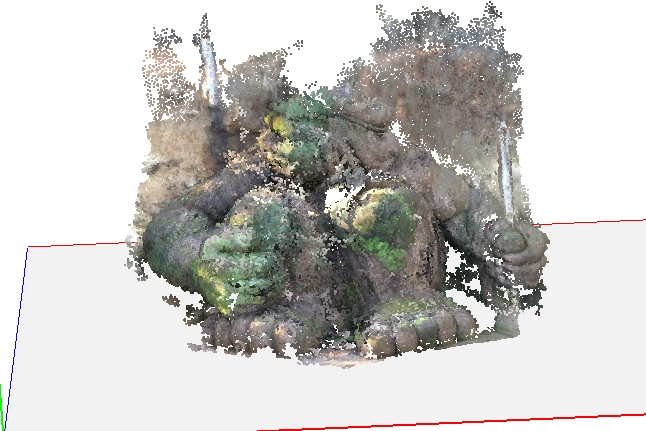
\includegraphics[width=0.40\linewidth]{figs/guerreirovisualsfmdmr.jpg}(a)
	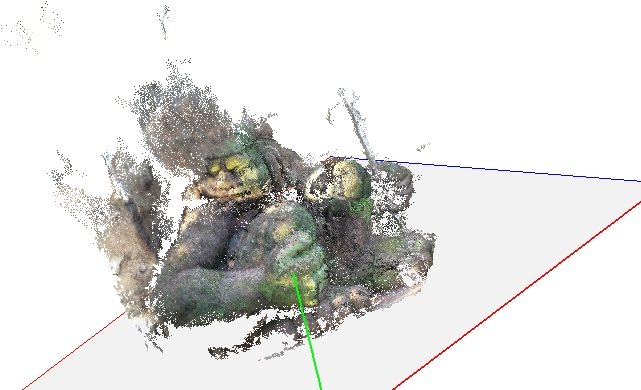
\includegraphics[width=0.50\linewidth]{figs/guerreirovisualsfmdmr2.jpg}(b)
	\legend{%
		Usando o software VisualSfM, em dois ângulos diferentes (a) e (b).
	}
		\source{
   	 O autor,
   	 2017.
   }\label{fig:reconstrucaoDensaIndioVisualSFM}
\end{figure}


%-------------------GALINHA A PARTIR DAQUI----------------------------------%

Com o objeto em ambiente fechado, conseguimos os resultados a seguir. 
Para o primeiro vídeo, convertido em 200 imagens, os tempos estão relatados na
Tabela~\ref{tab:temposSfM}.

\begin{table}[!h]
\caption{Tempos obtidos da reconstrução do objeto, com 200 imagens usando o VisualSfM}
\label{tab:temposSfM}
\begin{tabular}{|l|p{4.7cm}|}
\hline
Procedimento & Tempo (aprox.) \\ \hline
Carregamento de imagens & 50 segundos \\ \hline
Calcular pares correspondentes de \emph{features} & 2 horas e 40 minutos \\ \hline
Gerar a reconstrução esparsa do modelo & 2 minutos e 25 segundos \\ \hline
Gerar a reconstrução densa do modelo & 24 minutos \\ \hline
\end{tabular}
	\source{
   	 O autor,
   	 2017.
   }
\end{table}

A Figura~\ref{fig:reconstrucaoEsparsaVisualSFM} mostra o resultado da
reconstrução esparsa pelo algoritmo PBA. Nota-se que não é tão nítida como na reconstrução
densa, Figura~\ref{fig:reconstrucaoDensaVisualSFM}, dada a quantidade de ruídos
provenientes de outros objetos presentes na cena (o VisualSfM só identifica
objetos estáticos). Só é possível limpar a malha manualmente, pressionando a
tecla \texttt{F1} e selecionando a área desejada para ser deletada. Não é muito prático,
pois podemos excluir alguns pontos importantes. O ideal seria fazer esta limpeza
por meio de programas externos.

\newpage

\begin{figure}[!h]
	\centering
	\caption{%
	Reconstrução esparsa do objeto no VisualSfM com 200 imagens.
	}
		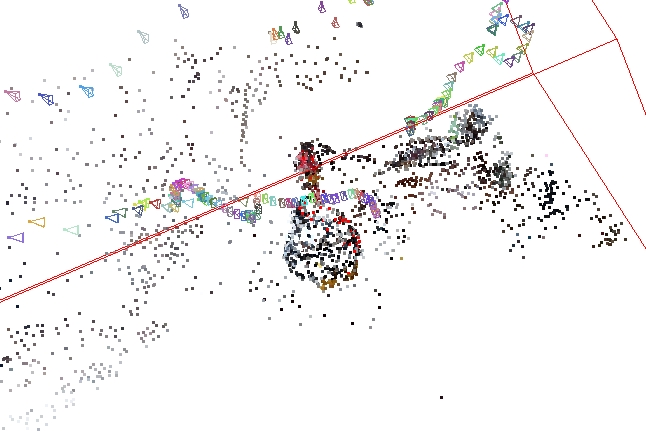
\includegraphics[width=0.8\linewidth]{figs/galinhasparsa.jpg}
	\source{
   	 O autor,
   	2017.
   }
	\label{fig:reconstrucaoEsparsaVisualSFM}
\end{figure}

\begin{figure}[!h]
	\centering
\caption{%
	Reconstrução densa do objeto no VisualSfM com 200 imagens.
	}	
	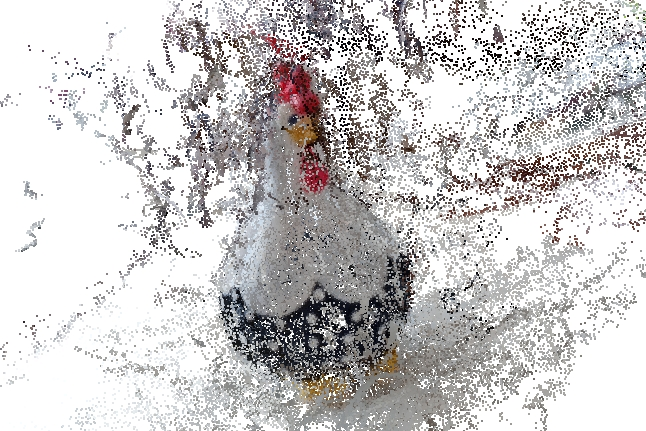
\includegraphics[width=0.8\linewidth]{figs/galinhadense.jpg}
	\source{
   	 O autor,
   	 2017.
   }
	\label{fig:reconstrucaoDensaVisualSFM}
\end{figure}

Outra reconstrução também foi realizada neste trabalho, utilizando os dois
vídeos do segundo objeto (cabaça), gerando 224 imagens, onde quando era usado um conjunto maior o programa
parava de funcionar por falta de memória, mesmo após ajustar parâmetros (como o
número de vizinhos, número de \emph{cores} do processador, \emph{level} do PMVS,
entre outros) para tentar melhorar esse problema. Portanto, o experimento seguiu da
forma: os tempos estão relatados na Tabela~\ref{tab:temposSfM224}.

\begin{table}[h!]
\caption{Tempos obtidos da reconstrução do objeto, com 224 imagens usando o VisualSfM}
\label{tab:temposSfM224}
\begin{tabular}{|l|p{4.7cm}|}
\hline
Procedimento & Tempo (aprox.) \\ \hline
Carregamento de imagens & 1 minuto \\ \hline
Calcular pares correspondentes de \emph{features} & 3 horas \\ \hline
Gerar a reconstrução esparsa do modelo & 3 minutos \\ \hline
Gerar a reconstrução densa do modelo & 32 minutos \\ \hline
\end{tabular}
	\source{
   	 O autor,
   	 2017.
   }
\end{table}

Percebe-se que não foi tão proveitoso (qualitativamente) usar mais imagens neste
caso; inclusive, o algoritmo perdeu a referência do objeto e gerou um segundo
modelo espelhado na reconstrução esparsa,
Figura~\ref{fig:reconstrucaoEsparsaVisualSFM224}, e, consequentemente, na
reconstrução densa,
Figuras~\ref{fig:reconstrucaoDensaVisualSFM2241} e~\ref{fig:reconstrucaoDensaVisualSFM2242}, o que gerou uma certa incoerência na reconstrução.

\begin{figure}[!h]
	\centering
\caption{%
	Reconstrução esparsa do objeto com 224 imagens no VisualSfM.
	%\cite{Cui:Theobalt:etal:PAMI2013,Pajdla:etal:ICCV2011}.
	}	
	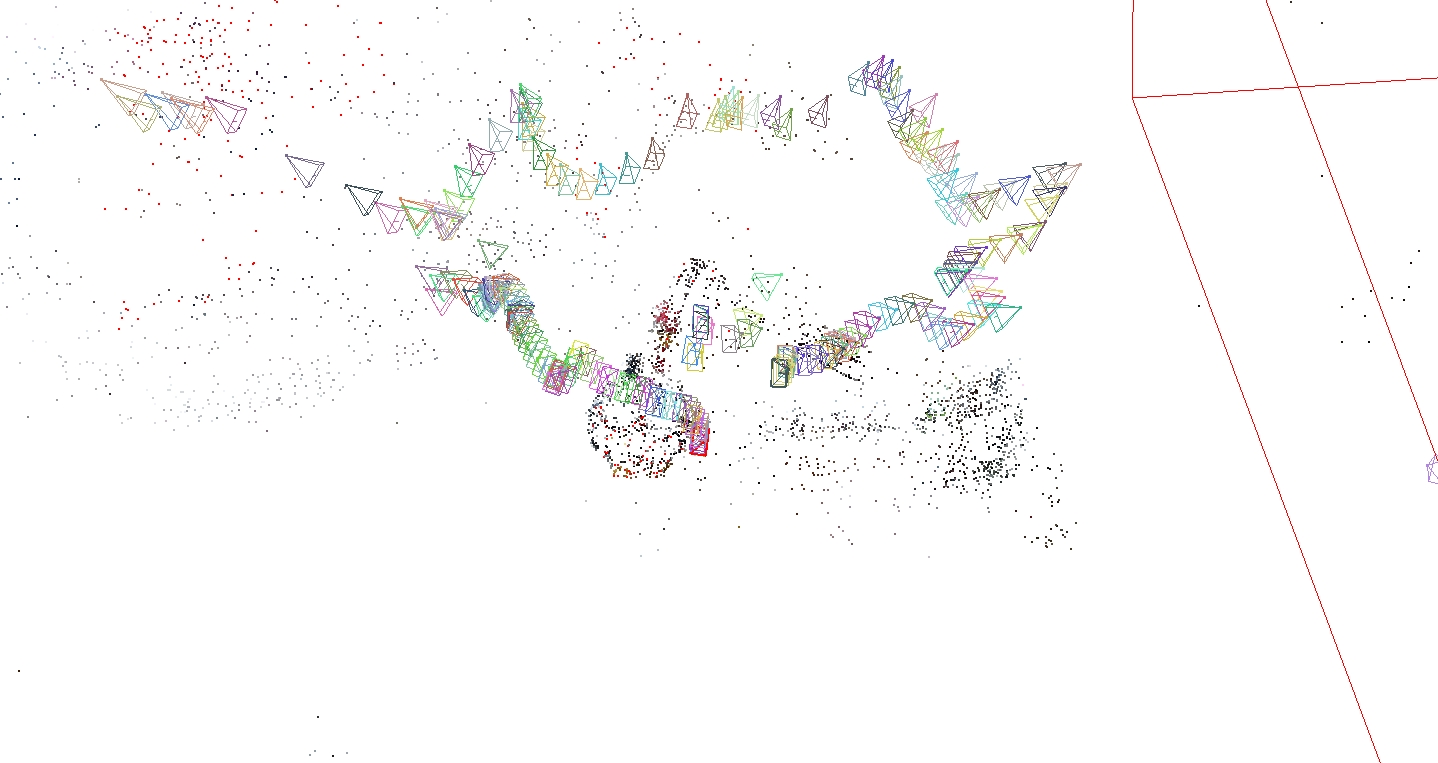
\includegraphics[width=\linewidth]{figs/perto_longe_esparsa.jpg}
	\source{
   	 O autor,
   	 2017.
   }
	\label{fig:reconstrucaoEsparsaVisualSFM224}
\end{figure}

\begin{figure}[!htpb]
	\centering
	\caption{Caso de falha do VisualSfM}
	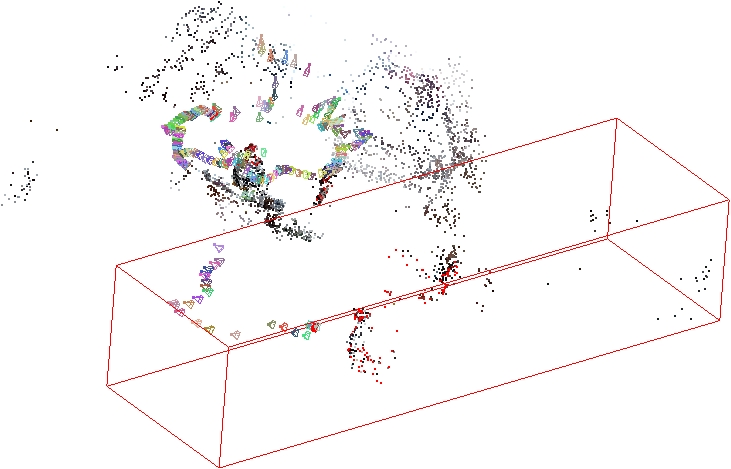
\includegraphics[width=0.9\linewidth]{figs/perto_longe_esparsa_2.jpg}
	\note{%
	 Foram gerados dois modelos refletidos esparsos do objeto a partir
  do conjunto inicial de 224 imagens, provavelmente, proveniente da falta de
  informações para estimar as câmeras.
	%\cite{Cui:Theobalt:etal:PAMI2013,Pajdla:etal:ICCV2011}.
	}
	\source{
   	 O autor,
   	 2017.
   }\label{fig:reconstrucaoEsparsaVisualSFM224:2}
\end{figure}

\clearpage

\begin{figure}[!h]
	\centering
	\caption{Resultado das reconstruções densas do objeto}
	{\label{fig:reconstrucaoDensaVisualSFM2241}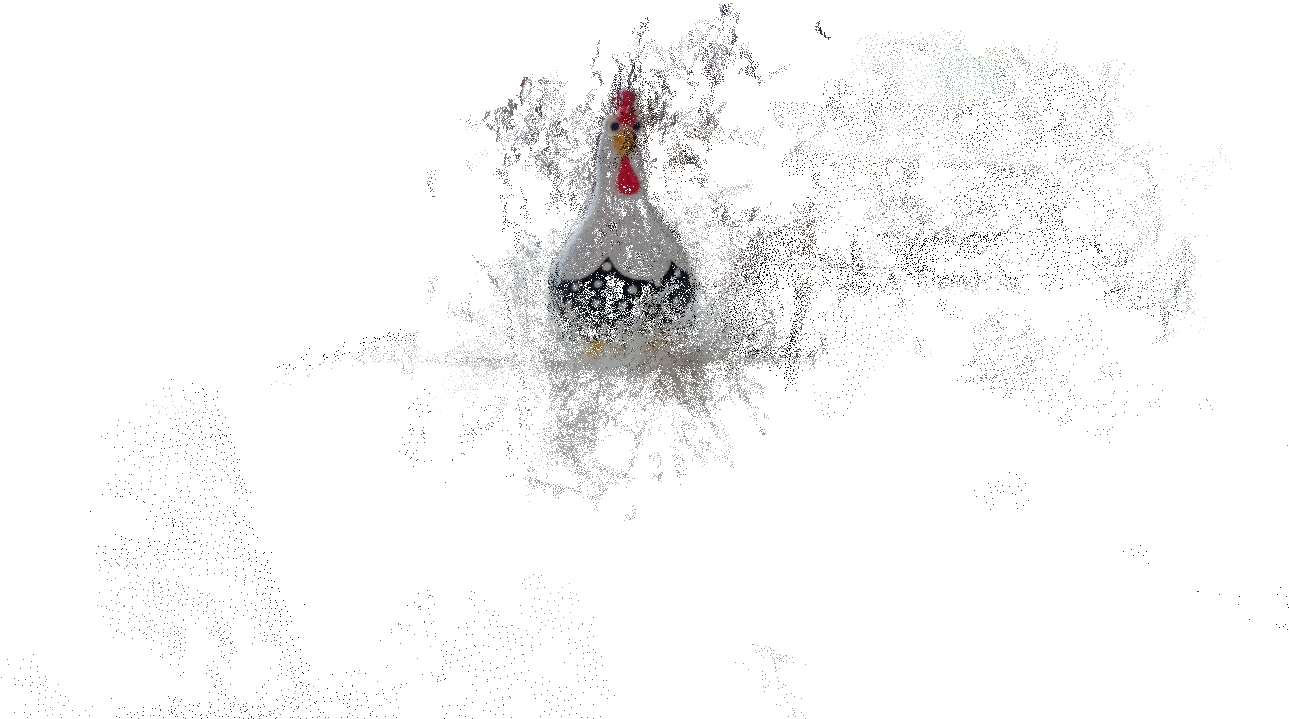
\includegraphics[width=\linewidth]{figs/galinhadense224.jpg}}(a)
	{\label{fig:reconstrucaoDensaVisualSFM2242}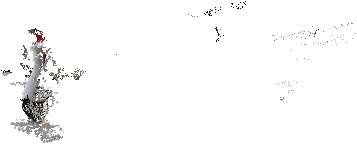
\includegraphics[width=\linewidth]{figs/galinhavisualsfm224.jpg}}(b)
	\legend{(a) - reconstrução densa do primeiro modelo;(b) - reconstrução densa do segundo modelo.
	}
	\note {%
	Reconstrução do objeto no VisualSFM com 224 imagens.
	}
	\source{
   	 O autor,
   	 2017.
   }
\end{figure}

%------------------ACABOU SFM---------------------------------------------%

\subsection{Resultados da reconstrução com o MVE}

A utilização do software é bem intuitiva, seja por linha de comando ou pela
interface gráfica (neste modo, fica mais fácil visualizar cada etapa da
reconstrução). O programa é amplamente configurável, podendo escolher a vizinhança, escala,
manter o mapa de profundidade, ver os dados \texttt{EXIF} de cada imagem, dentre
outras configurações.

\begin{figure}[!htpb]
	\centering
	\caption{Procedimento do MVE}
	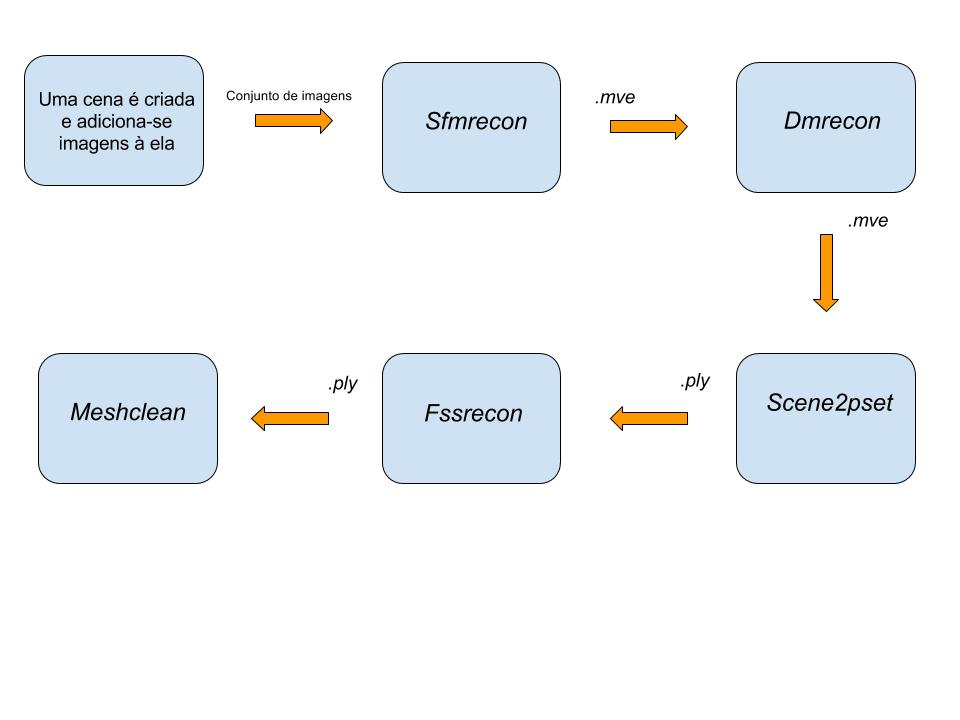
\includegraphics[width=0.5\linewidth]{figs/pipelineMVE.jpg}
	\note{%
	Processo de reconstrução usando o MVE por linha de comando: O \texttt{sfmrecon} executa os passos do SfM no conjunto de imagens e gera um arquivo \texttt{.mve} para cada imagem. Após isso, são associados mapas de profundidade a cada \texttt{.mve} com o \texttt{dmrecon}. Em seguida o \texttt{scene2pset} cria uma nuvem de pontos densa com a união de todas as amostras de todos os mapas de profundidade. O \texttt{fssrecon} executa o algoritmo de reconstrução de superfícies 3D e gera uma malha daquele objeto a ser reconstruído e, por fim, o \texttt{meshclean} limpa os ruídos do modelo e retira algumas triangulações defeituosas da etapa do \texttt{fssrecon}.
	}
	\source{
   	 O autor,
   	 2017.
   }
\end{figure}

Entretanto, para a aplicação proposta neste projeto, o MVE não é muito interessante,
visto que utiliza fortemente a informação \emph{a priori} das câmeras inseridas nas imagens
(\texttt{EXIF}) e, como as imagens empregadas na reconstrução são, tecnicamente,
vídeos cortados em determinados \emph{frames}, não é fácil obter essa informação
das câmeras~\ref{fig:mveexif}. Logo o, software não tem tanta aplicabilidade
neste caso, pois pode recair no problema dos parâmetros padrões adotados para as
câmeras não serem bons o suficiente para estes conjuntos de dados. A menos que
sejam tiradas fotos sequenciais de alguma escultura ou objeto que se deseja
gerar a reconstrução densa, pois dessa forma, as informações necessárias das
câmeras estarão armazenadas no \texttt{EXIF}. 

\begin{figure}[!htpb]
	\centering
	\caption{Extensão \texttt{EXIF}}
	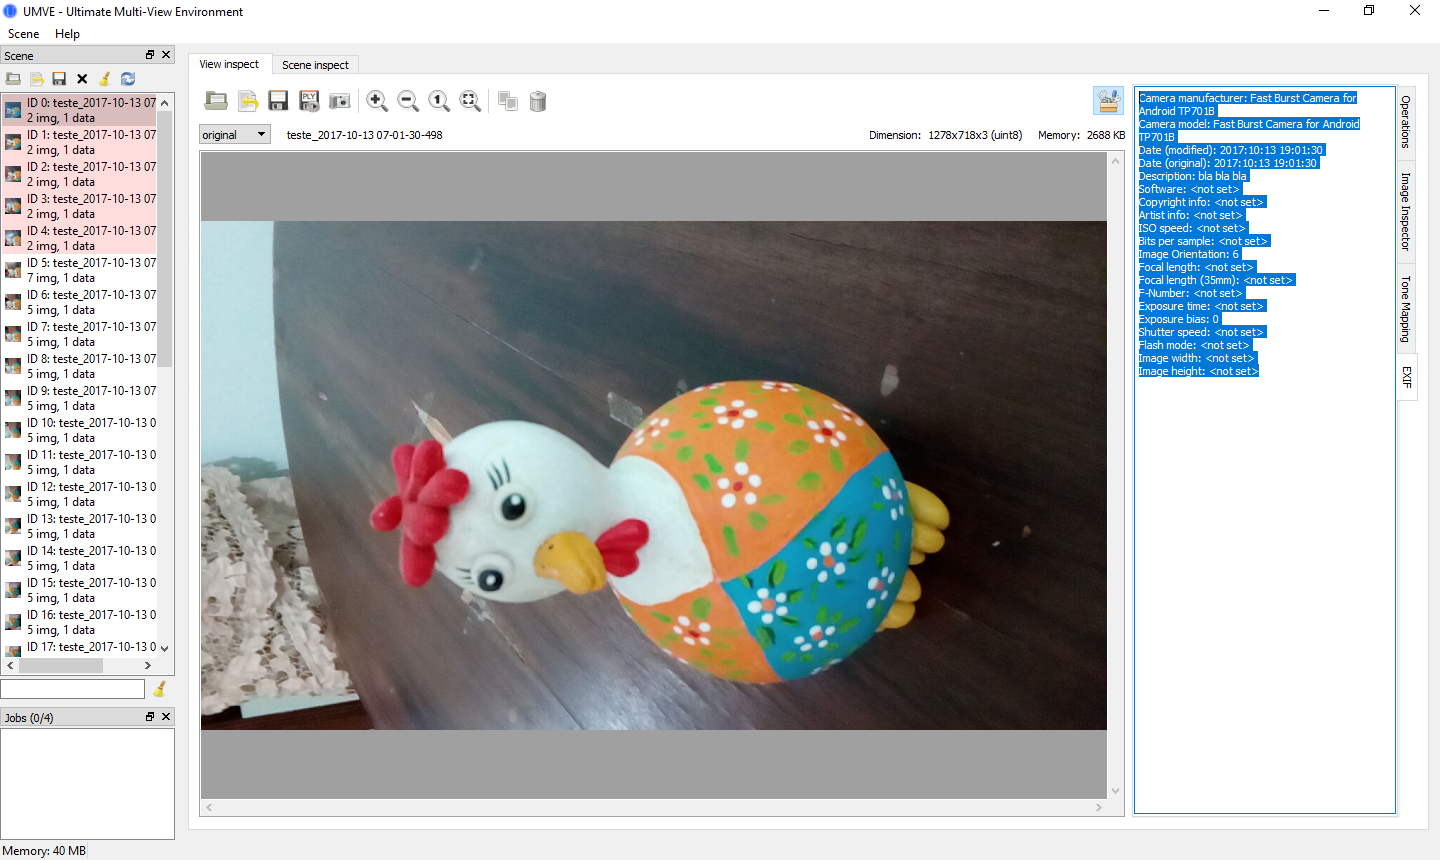
\includegraphics[width=0.35\linewidth]{figs/exifumve.png}(a)
	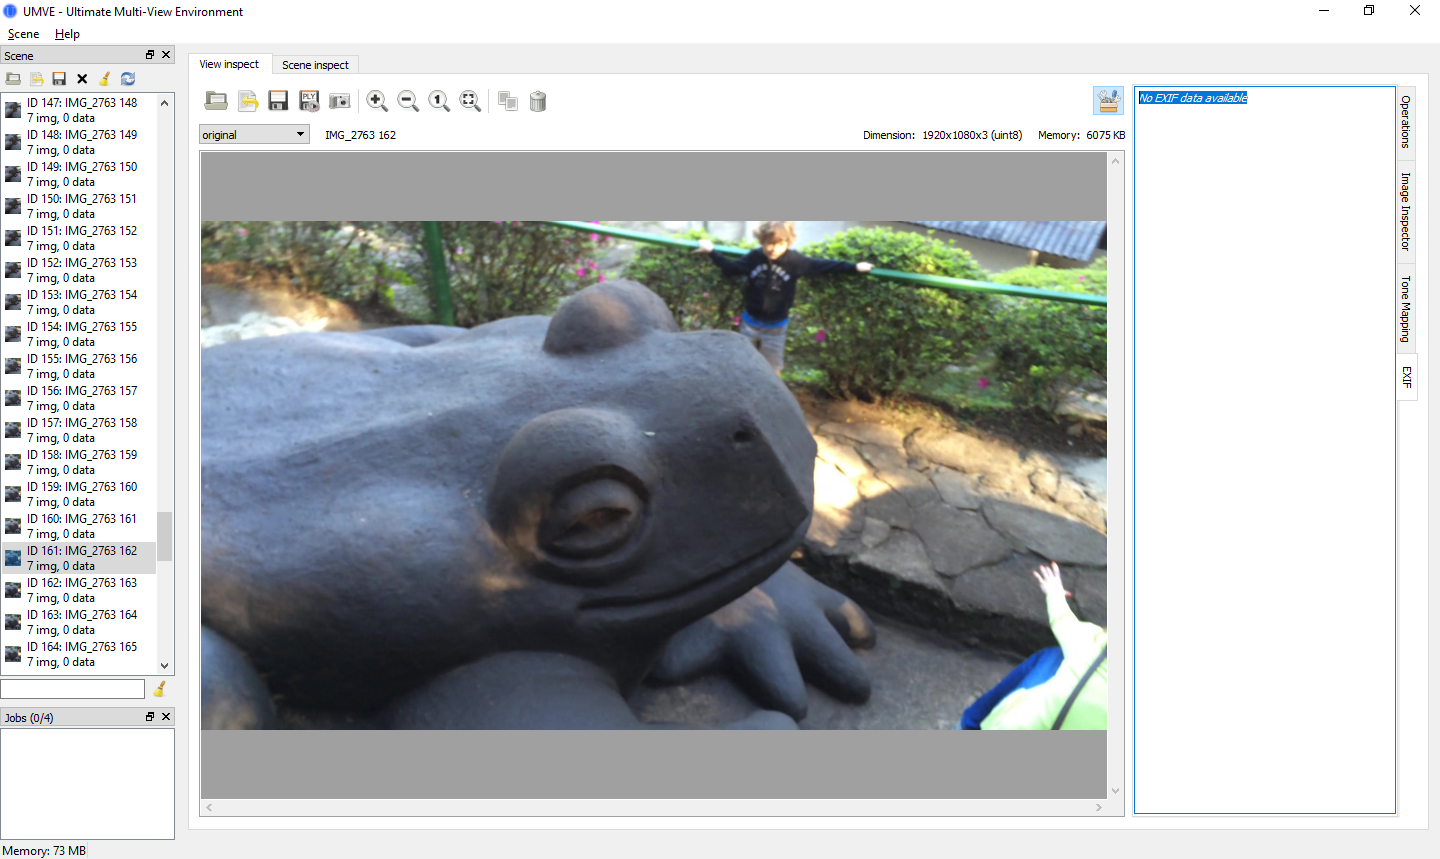
\includegraphics[width=0.35\linewidth]{figs/exifsemumve.png}(b)
	\legend{%
  (a) - imagem com dados na extensão \texttt{EXIF}
  (em azul); (b) - um frame de um vídeo, que não
  possui os dados das câmeras (em azul).
	%\cite{Cui:Theobalt:etal:PAMI2013,Pajdla:etal:ICCV2011}.
	}
	\source{
   	 O autor,
   	 2017.
   }\label{fig:mveexif}
\end{figure} 

Foi gerada uma reconstrução no MVE de um vídeo gravado de uma escultura no Jardim do
Nêgo. O  vídeo foi reduzido a \emph{frames} de onde foram selecionadas 200 imagens base,
com os parâmetros de câmera gerados pelo próprio software, mesmo sem o
\texttt{EXIF} para ajudar na estimativa inicial. 
A partir disso, foram executados todos os passos de uma reconstrução utilizando o
MVE, de forma que foram utilizadas as duas opções, tanto por linha de comando,
quanto pela interface gráfica (UMVE).

Pela interface gráfica, o processo todo de reconstrução foi rápido (cerca de 30
minutos), Figura~\ref{fig:UMVEdense}, ao passo que por linha de comando, levou cerca de
11 horas e 30 minutos. Portanto, vamos nos atentar somente à reconstrução por
linha de comando, onde, resumindo, tivemos os resultados na Tabela~\ref{tab:mveSapo}. 
O UMVE não sinaliza quando o processo em execução termina; a explicação
para essa discrepância no tempo é devido à execução de outro comando, sobrepondo
o que já estava sendo executado, sem que o primeiro tivesse terminado.

\newpage

\begin{figure}[!h]
	\centering
	\caption{Reconstrução usando a interface gráfica do MVE}
	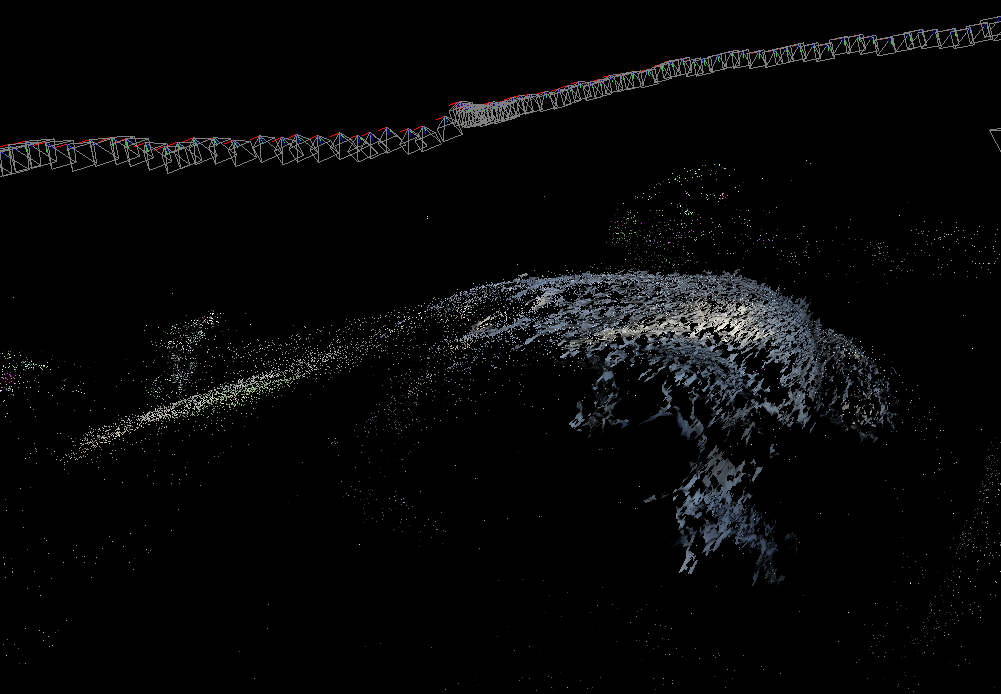
\includegraphics[width=\linewidth]{figs/umvedense.png}
	\note{%
  Reconstrução final via UMVE; percebe-se que alguns pontos não foram
  considerados, mas o resultado geral foi uma nuvem de pontos mais densa.
  %\cite{Cui:Theobalt:etal:PAMI2013,Pajdla:etal:ICCV2011}.
	}
	\source{
   	 O autor,
   	 2017.
   }\label{fig:UMVEdense}
\end{figure} 

\begin{table}[!htpb]
\centering
\caption{Tempos obtidos usando o MVE em um conjunto de dados do Jardim do Nêgo}
\label{tab:mveSapo}
\begin{tabular}{|l|l|}
\hline
Comando            & Tempo (aprox.)    \\ \hline
\texttt{sfmrecon}  & 1 minuto e 28 segundos     \\ \hline
\texttt{dmrecon}   & 4 horas \\ \hline
\texttt{scene2pset} & 10 minutos    \\ \hline
\texttt{fssrecon}  & 7 horas \\ \hline
\texttt{meshclean} & 1 minuto     \\ \hline
\end{tabular}
	\source{
   	 O autor,
   	 2017.
   }
\end{table}

Na reconstrução por linha de comando também é possível visualizar em qual etapa
da execução o algoritmo está (Figura~\ref{fig:passosMVE}), configurar alguns
parâmetros e inclusive mostrar a porcentagem de progresso do comando em
execução. Foram executados os comandos declarados nesta seção.  O
\texttt{sfmrecon} demorou cerca de 1 minuto e meio. %\ref{fig:MVESfM}. 

\clearpage

\begin{figure}[!htpb]
	\centering
	\caption{Linha de comandos do \texttt{sfmrecon}}
	\subfloat[]{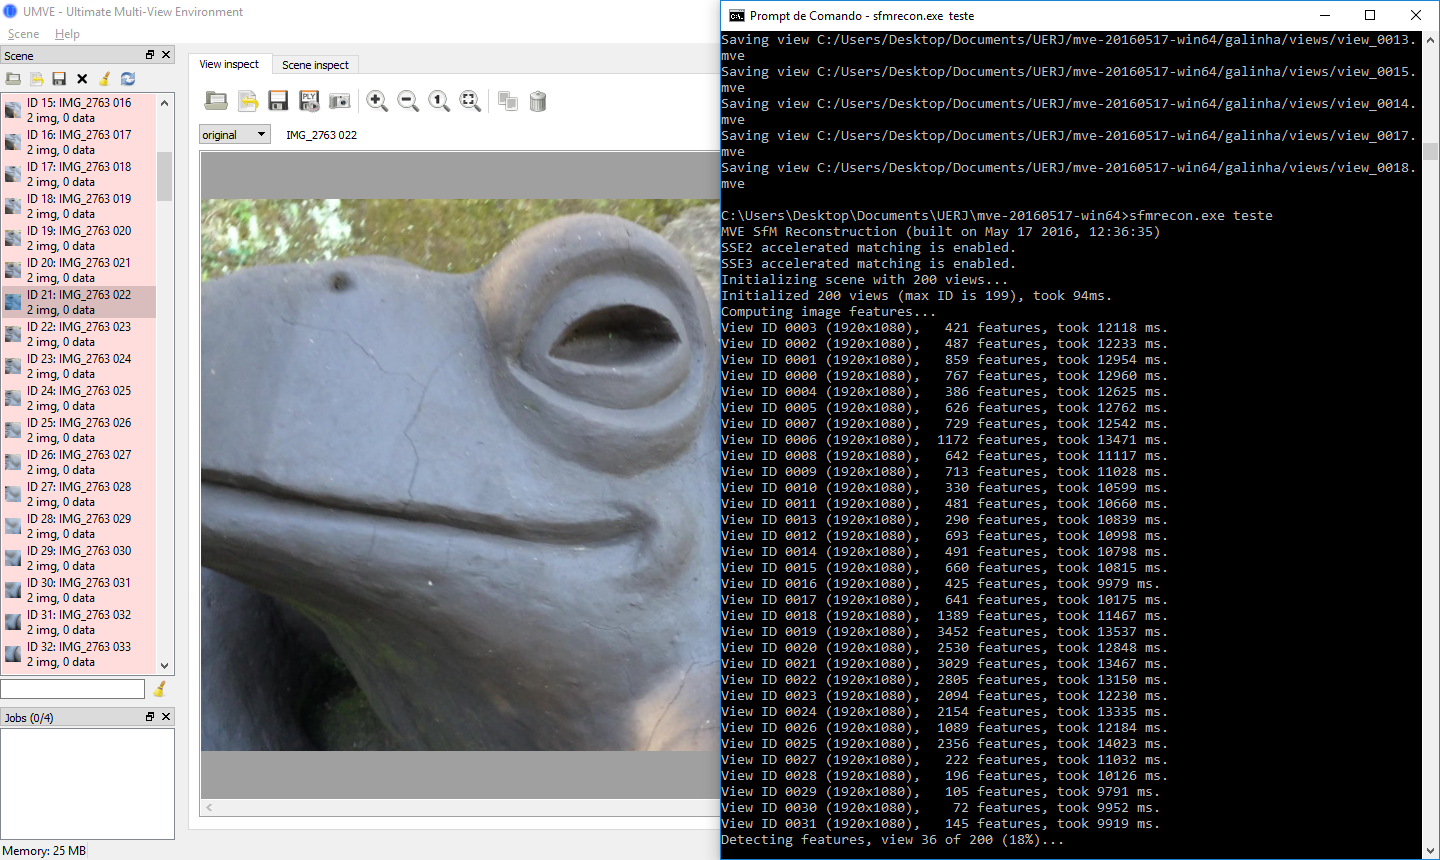
\includegraphics[width=0.5\linewidth]{figs/umve2sfm.png}}
	\subfloat[]{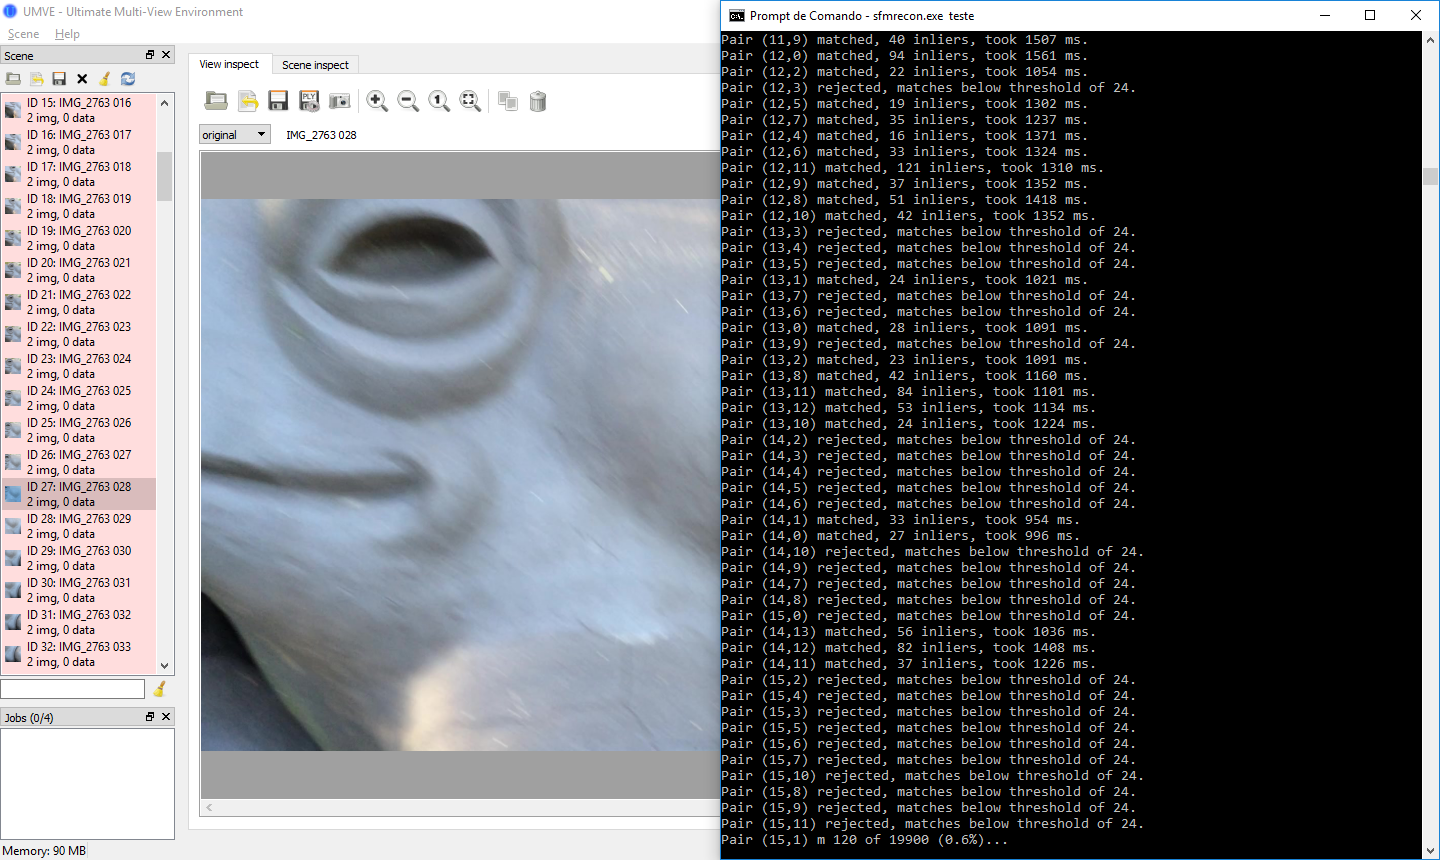
\includegraphics[width=0.5\linewidth]{figs/umve3sfmfeature.png}}
	\note{%
  Processos dentro do comando \texttt{sfmrecon}, onde (a) estão sendo detectadas
  as \emph{features} do conjunto de imagens e em (b) está computado o
  \emph{pairwise matching}.
  %\cite{Cui:Theobalt:etal:PAMI2013,Pajdla:etal:ICCV2011}.
  }
  	\source{
   	 O autor,
   	 2017.
   }\label{fig:passosMVE}
\end{figure} 

% \begin{figure}[h!]
% 	\centering
% 	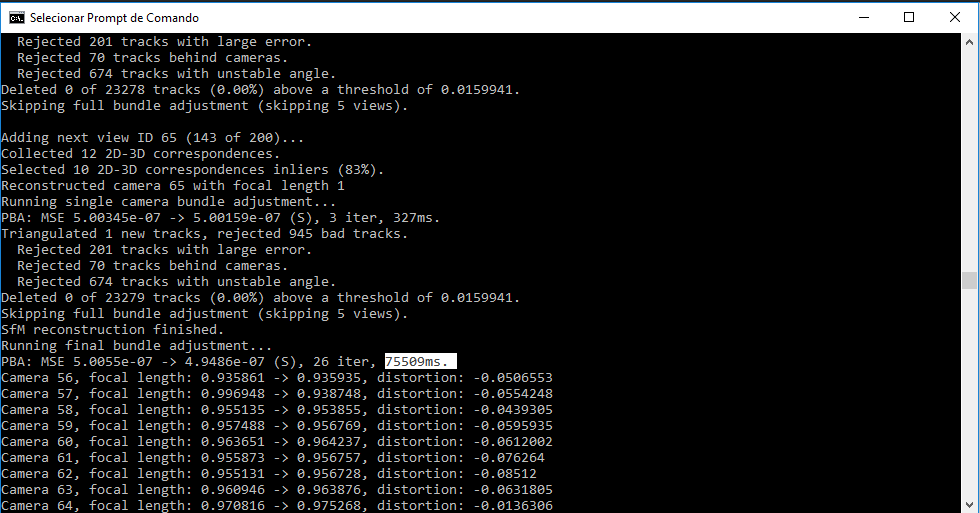
\includegraphics[width=0.65\linewidth]{figs/sfmmve.png}
% 	\caption{%
% 	Término do comando \emph{sfmrecon}, onde demorou cerca de 1 minuto e meio (75509 milisegundos).
% 	%\cite{Cui:Theobalt:etal:PAMI2013,Pajdla:etal:ICCV2011}.
% 	}\label{fig:MVESfM}
% \end{figure}

O próximo comando, \texttt{dmrecon} demorou cerca de 4 horas, usando como
configuração um nível L2, com 20 vizinhos. %\ref{fig:MVEDenseRecon}.  
Usando um
nível L0, o algoritmo rodou durante 6 horas aproximadamente e foi cancelado
devido à demora na execução. 

% \begin{figure}[!h]
% 	\centering
% 	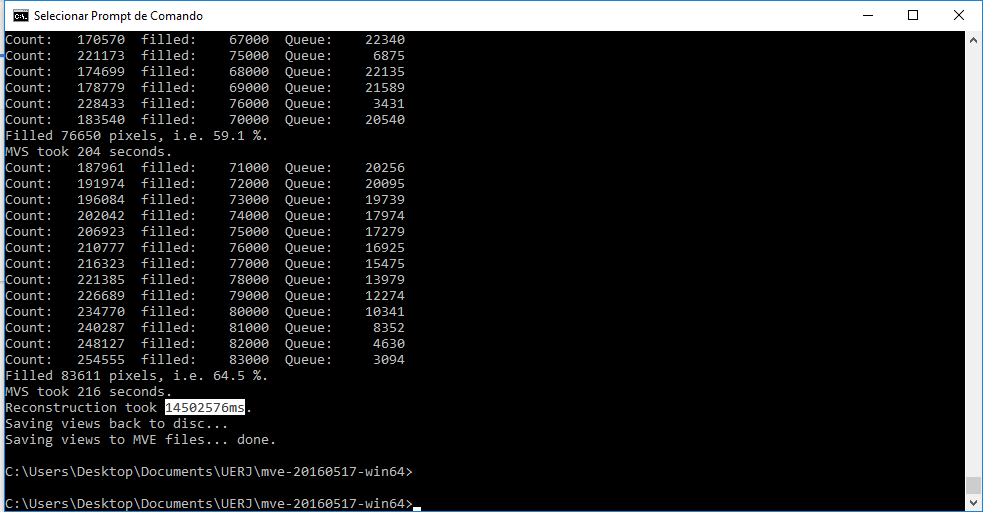
\includegraphics[width=0.8\linewidth]{figs/umvetempo.png}
% 	\caption{%
% 	Término do comando \emph{dmrecon}, onde demorou cerca de 4 horas (14502576 milisegundos).
% 	%\cite{Cui:Theobalt:etal:PAMI2013,Pajdla:etal:ICCV2011}.
% 	}\label{fig:MVEDenseRecon}
% \end{figure} 

Usando o \texttt{scene2pset}, é necessário especificar em qual nível estamos
reconstruindo e também uma saída válida. Por exemplo: \texttt{scene2pset.exe -Fnivel
cena output}, onde o nível (escala do tamanho das imagens) poderá ser um 0 (-F0), 1 (-F1) e assim por diante; a
cena é o \emph{input} e o \emph{output} é um arquivo de extensão configurável,
neste caso \texttt{.ply} %\ref{fig:MVEscene2pset}. 
Este comando foi rápido, demorou
cerca de 10 minutos, levando em conta todos os níveis.

% \begin{figure}[!h]
% 	\centering
% 	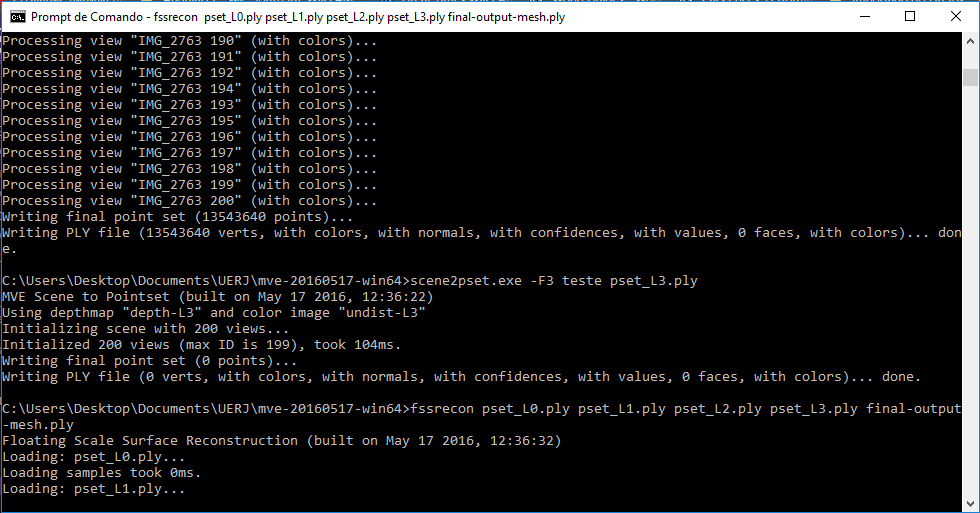
\includegraphics[width=0.8\linewidth]{figs/mvemesh.png}
% 	\caption{%
% 	Execução dos comandos \emph{scene2pset}, nos níveis -F0, -F1, -F2 e -F3.
% 	%\cite{Cui:Theobalt:etal:PAMI2013,Pajdla:etal:ICCV2011}.
% 	}\label{fig:MVEscene2pset}
% \end{figure} 

Para juntar todos os níveis do \texttt{scene2pset}, foi usado o \texttt{fssrecon},
que gera uma única reconstrução. Este processo demorou bastante, cerca de 7
horas e teve como resultado a malha da Figura~\ref{fig:MVEFSSRMesh}.
Porfim, basta limpar a malha atual com o comando \texttt{meshclean}, onde foi
obtido o resultado~\ref{fig:MVEMeshClean}.

% \begin{figure}[!h]
% 	\centering
% 	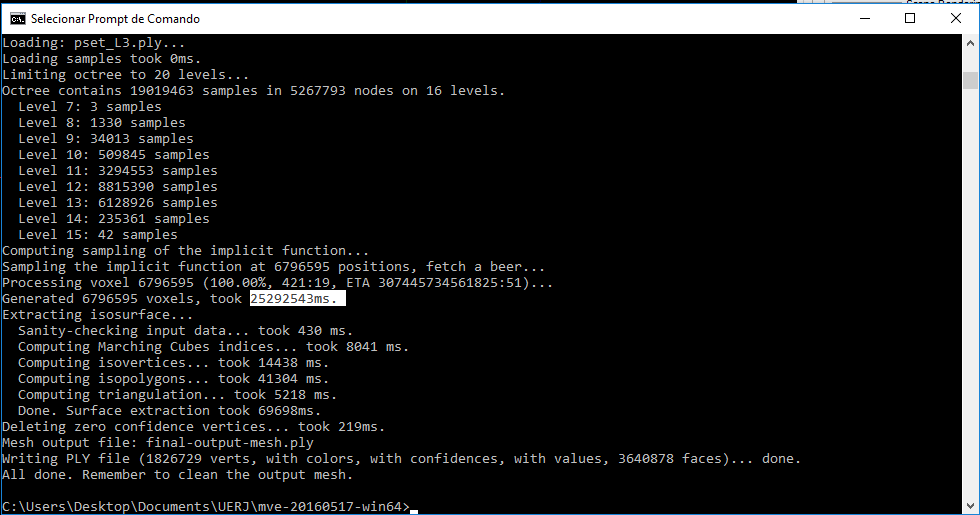
\includegraphics[width=0.8\linewidth]{figs/mvemeshtempo2.png}
% 	\caption{%
% 	Progressão do comando \emph{fssrecon}, onde possui o ETA -- \emph{Estimated Time of Arrival}.
% 	%\cite{Cui:Theobalt:etal:PAMI2013,Pajdla:etal:ICCV2011}.
% 	}\label{fig:MVEFSSR}
% \end{figure} 

\begin{figure}[!h]
	\centering
	\caption{%
	Malha com ruídos proveniente do comando \texttt{fssrecon}.
	}
	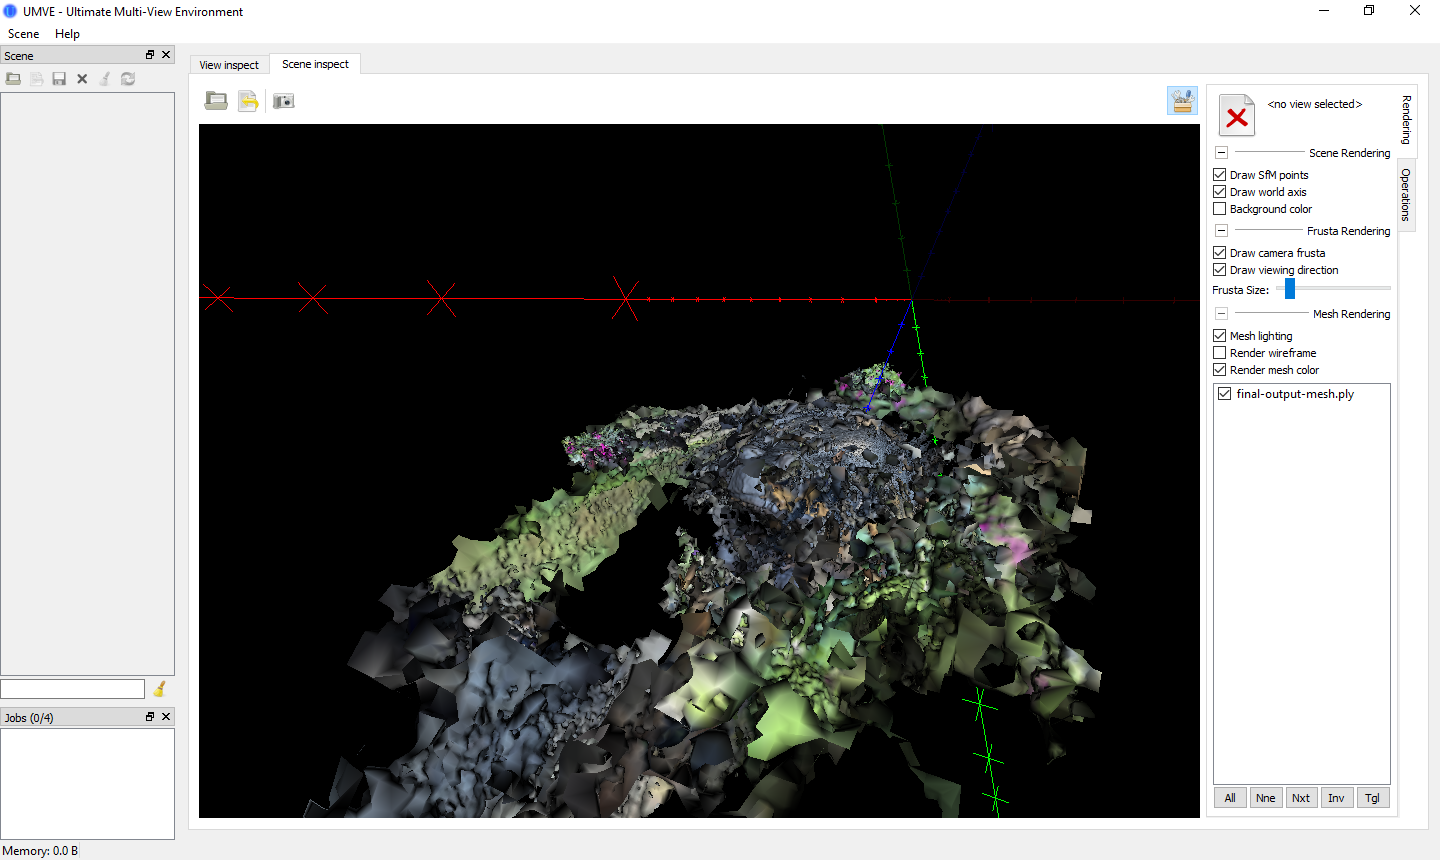
\includegraphics[width=0.95\linewidth]{figs/mvemeshout.png}
	\source{
   	 O autor,
   	 2017.
   }
   \label{fig:MVEFSSRMesh}
\end{figure} 

\begin{figure}[!h]
	\centering
	\caption{%
	Resultado final, após a remoção dos ruídos da malha.
	%\cite{Cui:Theobalt:etal:PAMI2013,Pajdla:etal:ICCV2011}.
	}
	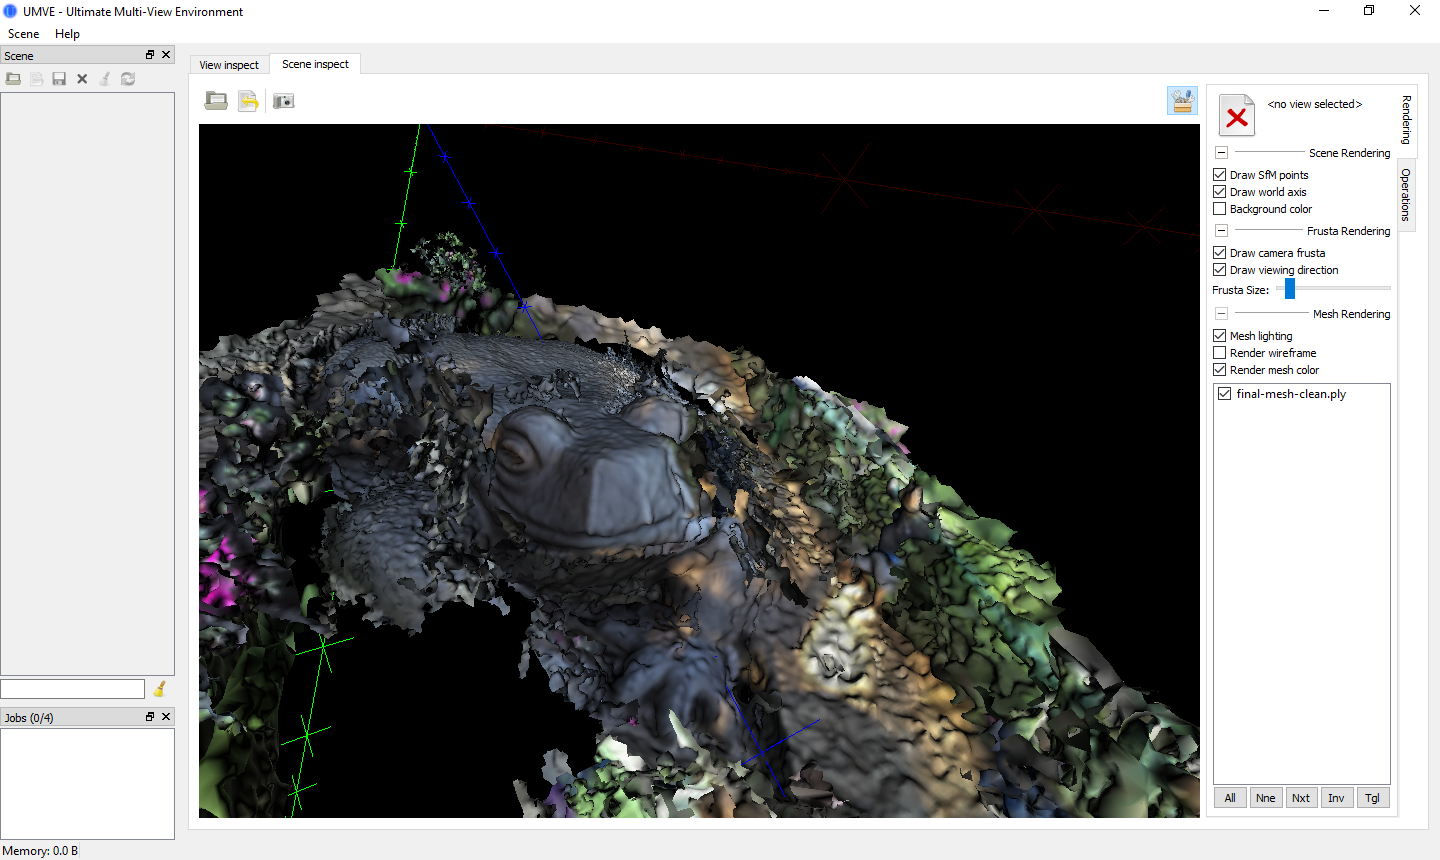
\includegraphics[width=1\linewidth]{figs/mvemeshclean.png}
	\source{
   	 O autor,
   	 2017.
   }
   \label{fig:MVEMeshClean}
\end{figure} 

\newpage

Para comparação, usou-se o mesmo objeto utilizado na reconstrução do VisualSfM (a
galinha) e foi feito o passo a passo com o MVE: com a interface gráfica (UMVE),
criou-se uma nova cena inserido-se, primeiramente, as 200 fotos do objeto. Em
seguida, utilizando as linhas de comando do MVE, foi feito o procedimento padrão
de reconstrução do software. Foram obtidos os resultados na Tabela~\ref{tab:galinha200mve}.

\begin{table}[!h]
\centering
\caption{Tempos obtidos usando o MVE em um conjunto de dados em ambiente interno com 200 imagens}
\label{tab:galinha200mve}
\begin{tabular}{|l|l|}
\hline
Comando            & Tempo (aprox.)         \\ \hline
\texttt{sfmrecon}  & 6 minutos   \\ \hline
\texttt{dmrecon}   & 1 hora \\ \hline
\texttt{scene2pset} & 5 minutos   \\ \hline
\texttt{fssrecon}  & 29 minutos \\ \hline
\texttt{meshclean} & 45 segundos    \\ \hline
\end{tabular}
	\source{
   	 O autor,
   	 2017.
   }
\end{table}

% \begin{figure}[!h]
% 	\centering
% 	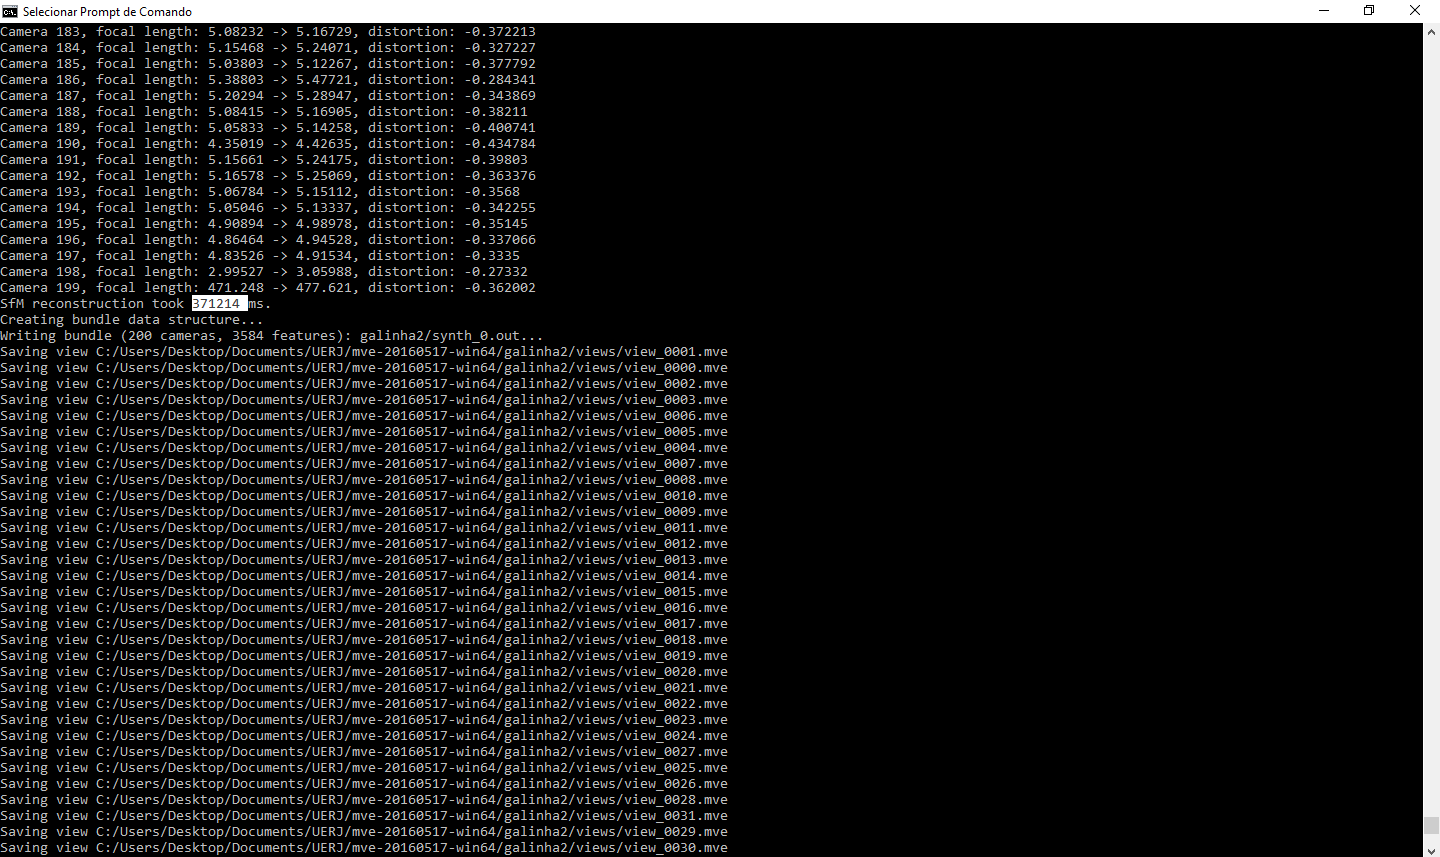
\includegraphics[width=0.5\linewidth]{figs/galinhalongesfmreconmve.png}
% 	\caption{%
% 	Tempo gasto da etapa \emph{sfmrecon} do MVE
% 	}\label{fig:sfmrecon1}
% \end{figure}

% \begin{figure}[!h]
% 	\centering
% 	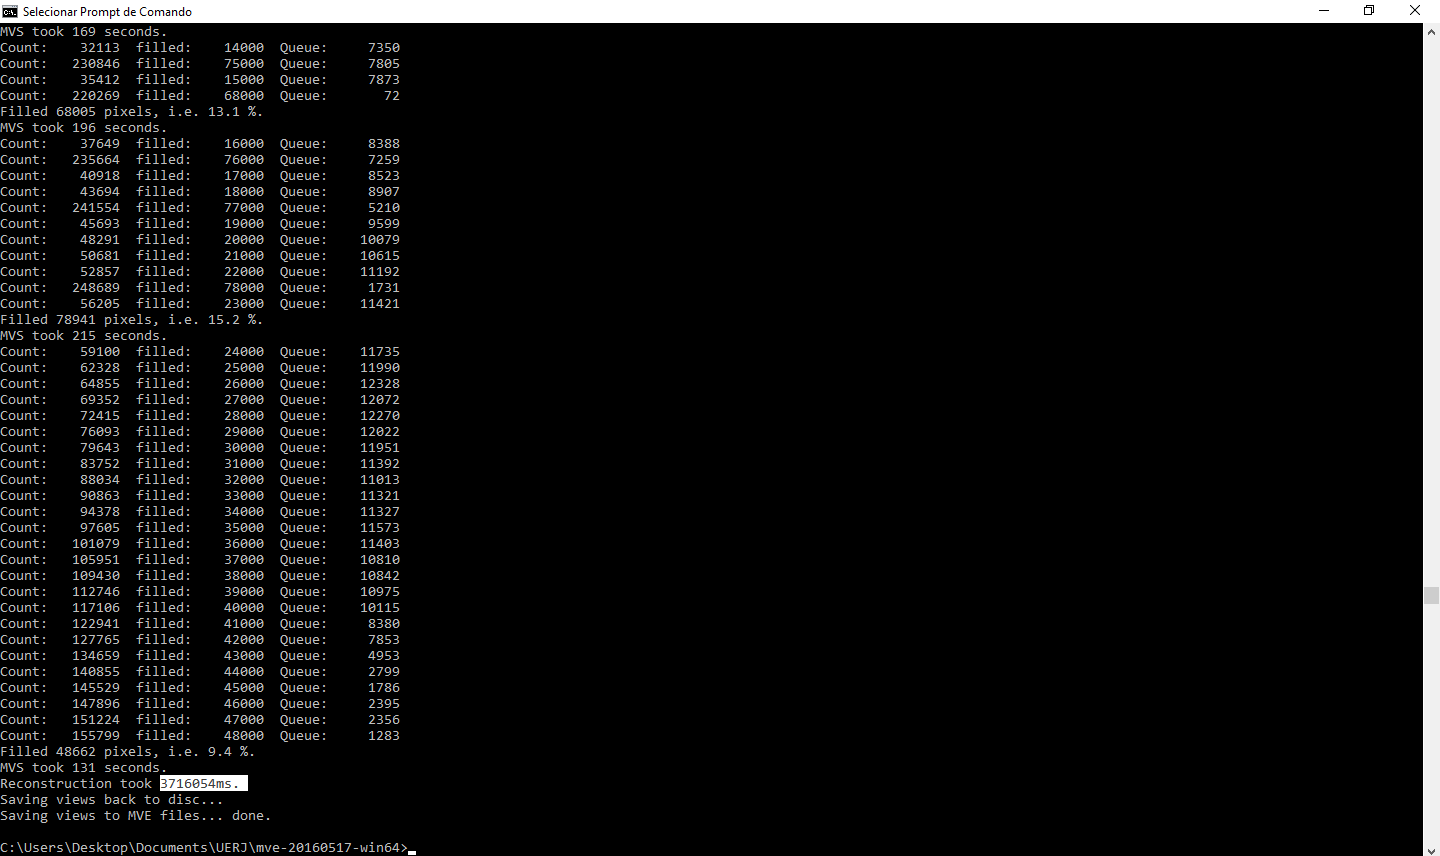
\includegraphics[width=0.5\linewidth]{figs/galinhadmreconmve.png}
% 	\caption{%
% 	Tempo da etapa \emph{dmrecon} do MVE
% 	%\cite{Cui:Theobalt:etal:PAMI2013,Pajdla:etal:ICCV2011}.
% 	}\label{fig:dmrecon1}
% \end{figure}

% \begin{figure}[!h]
% 	\centering
% 	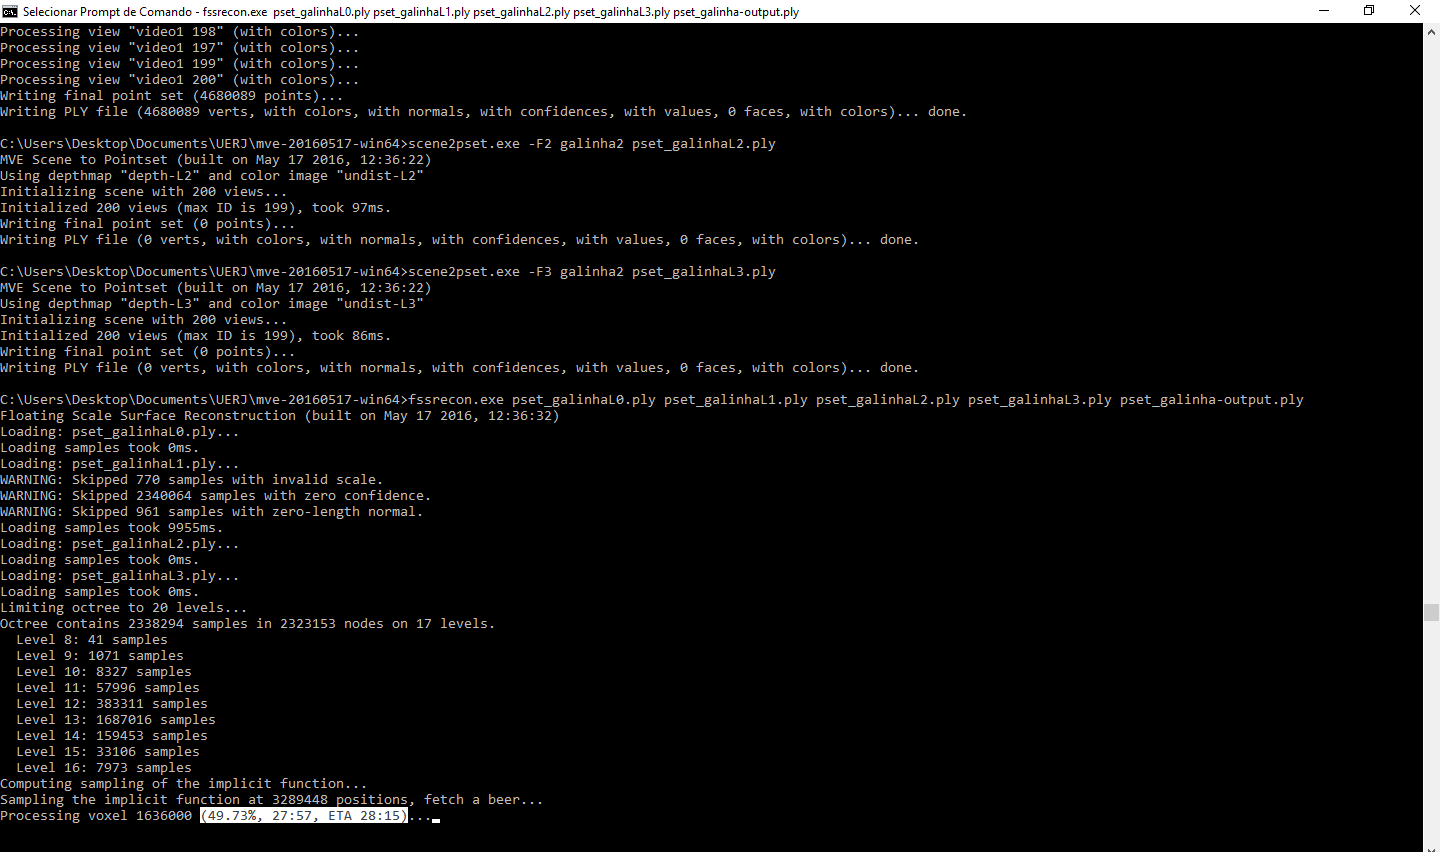
\includegraphics[width=0.7\linewidth]{figs/mvefssrecongalinha.png}
% 	\caption{%
% 	Tempo da etapa \emph{fssrecon} do MVE
% 	%\cite{Cui:Theobalt:etal:PAMI2013,Pajdla:etal:ICCV2011}.
% 	}\label{fig:fssrecon}
% \end{figure}

 \begin{figure}[!h]
 	\centering	
 	\caption{Resultado da etapa \texttt{fssrecon} do MVE}
 	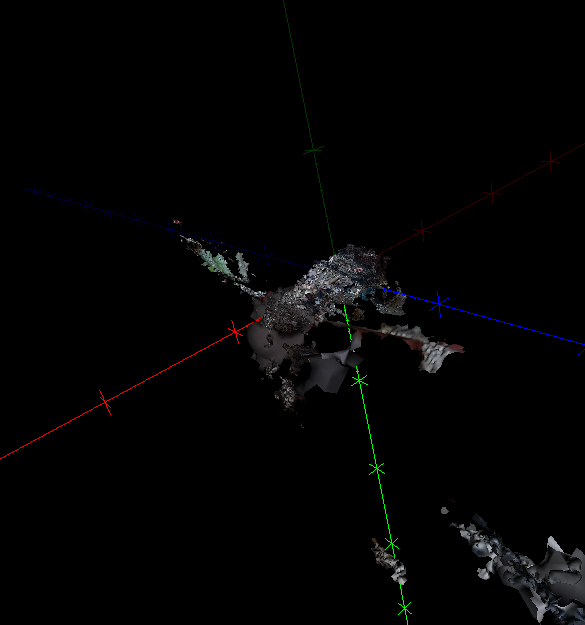
\includegraphics[width=0.7\linewidth]{figs/galinhadmr.png}
 	\source{
 	O autor, 2017.
 	}
 	\label{fig:galinhaFssr}
 \end{figure}

\newpage

\begin{figure}[!h]
	\centering
		\caption{%
	Resultado da etapa \texttt{meshclean}, da etapa anterior \ref{fig:galinhaFssr}
	%\cite{Cui:Theobalt:etal:PAMI2013,Pajdla:etal:ICCV2011}.
	}
	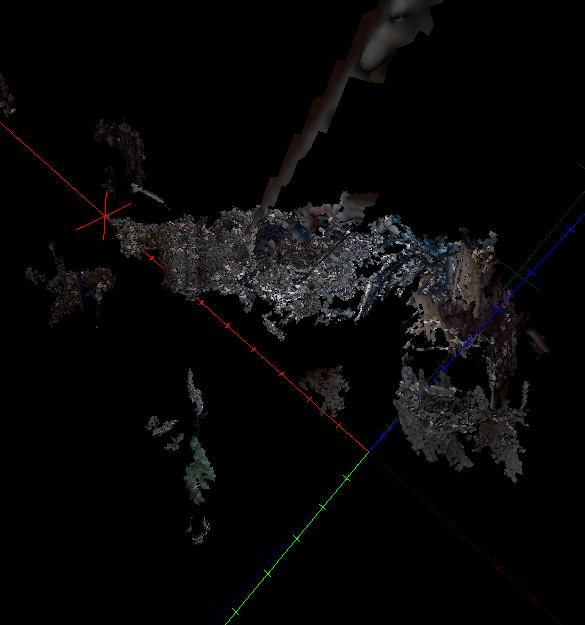
\includegraphics[width=0.7\linewidth]{figs/galinhameshclean.png}
	\source{
   	 O autor,
   	 2017.
   }
   \label{fig:galinhaMeshClean}
\end{figure}

A etapa de \texttt{scene2pset} demorou cerca de 20 segundos (total). Porém
a reconstrução não foi satisfatória, o software se confundiu, e
não conseguiu obter os parâmetros corretos das câmeras utilizadas. A partir
disso, o erro se propagou e gerou a reconstrução da Figura~\ref{fig:galinhaMeshClean}.  Rodamos também com as 224 fotos, mas só foi possível
executar o passo \texttt{sfmrecon}, pois o MVE não
conseguiu rodar o comando \texttt{dmrecon} provavelmente o SIFT falhou na correspondências entre as imagens, e não gerou nenhum
resultado para a continuação do algoritmo.%, Figura~\ref{fig:galinhaDMR224}.

% \begin{figure}[!h]
% 	\centering
% 	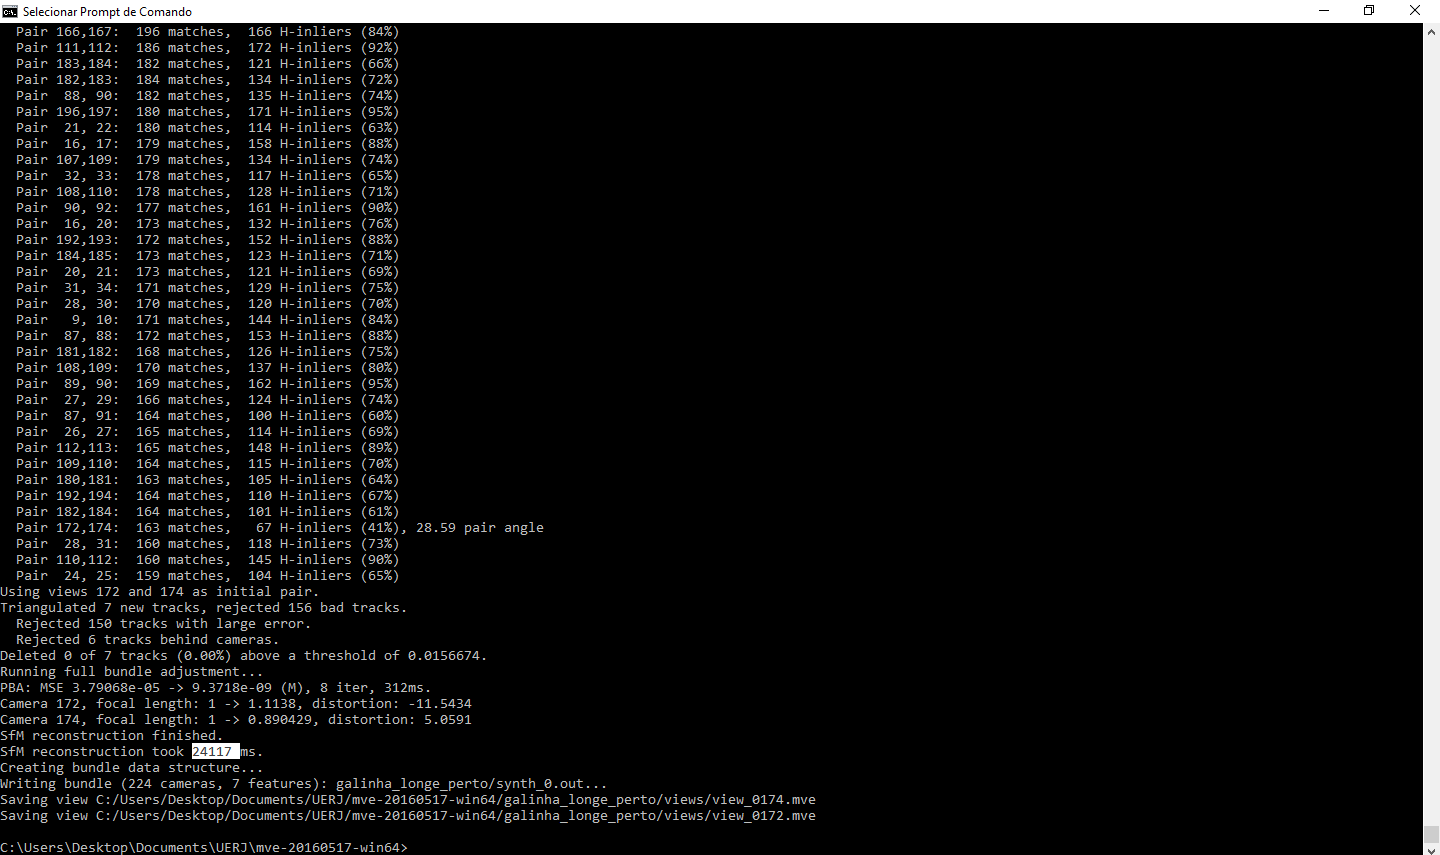
\includegraphics[width=0.5\linewidth]{figs/mvesfmrecongalinhapertolonge.png}
% 	\caption{%
% 	Resultado da etapa \emph{sfmrecon}, com todas as imagens
% 	%\cite{Cui:Theobalt:etal:PAMI2013,Pajdla:etal:ICCV2011}.
% 	}\label{fig:galinhaSfM224}
% \end{figure}

% \begin{figure}[!h]
% 	\centering
% 	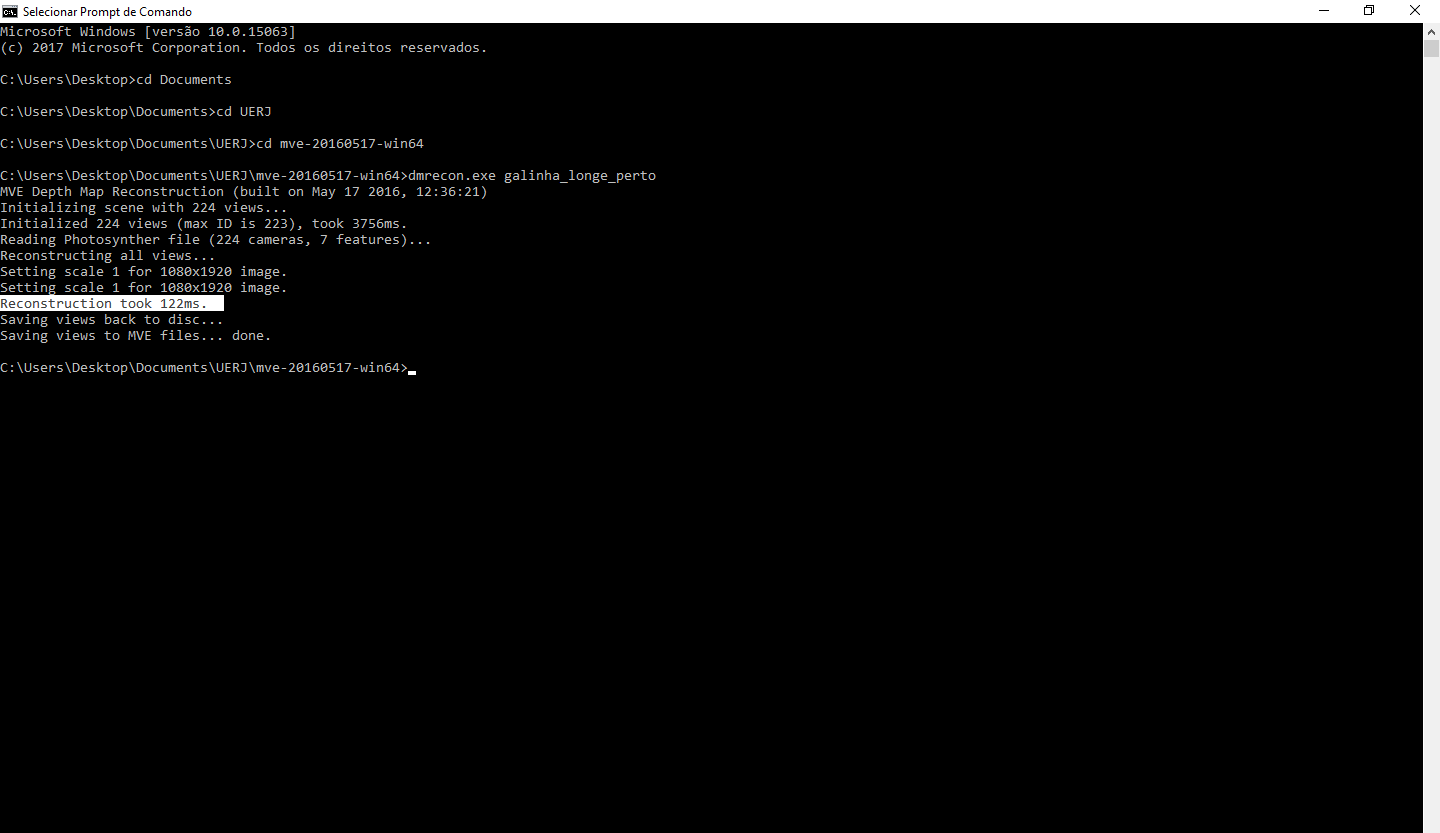
\includegraphics[width=0.5\linewidth]{figs/mvedmrecongalinhapertolonge.png}
% 	\caption{%
% 	Resultado da etapa \emph{dmrecon}, com todas as imagens
% 	%\cite{Cui:Theobalt:etal:PAMI2013,Pajdla:etal:ICCV2011}.
% 	}\label{fig:galinhaDMR224}
% \end{figure}

%Utilizando o Skanect versão gratuita, obtemos os seguintes resultados...%

\subsection{Resultados da reconstrução com o Sense}
Para a reconstrução com o Kinect, utilizamos uma ferramenta de escaneamento que utiliza o mesmo princípio do Kinect versão 1 (baseado em luz estruturada): o Sense versão 1~\cite{3DSystems}.

Seu formato facilita o manuseio do scanner para conseguirmos realizar uma boa varredura (figuras~\ref{fig:fotoSense0}, \ref{fig:fotoSense1}).

\begin{figure}[!h]
	\centering
	\caption{Caixa do Sense}
	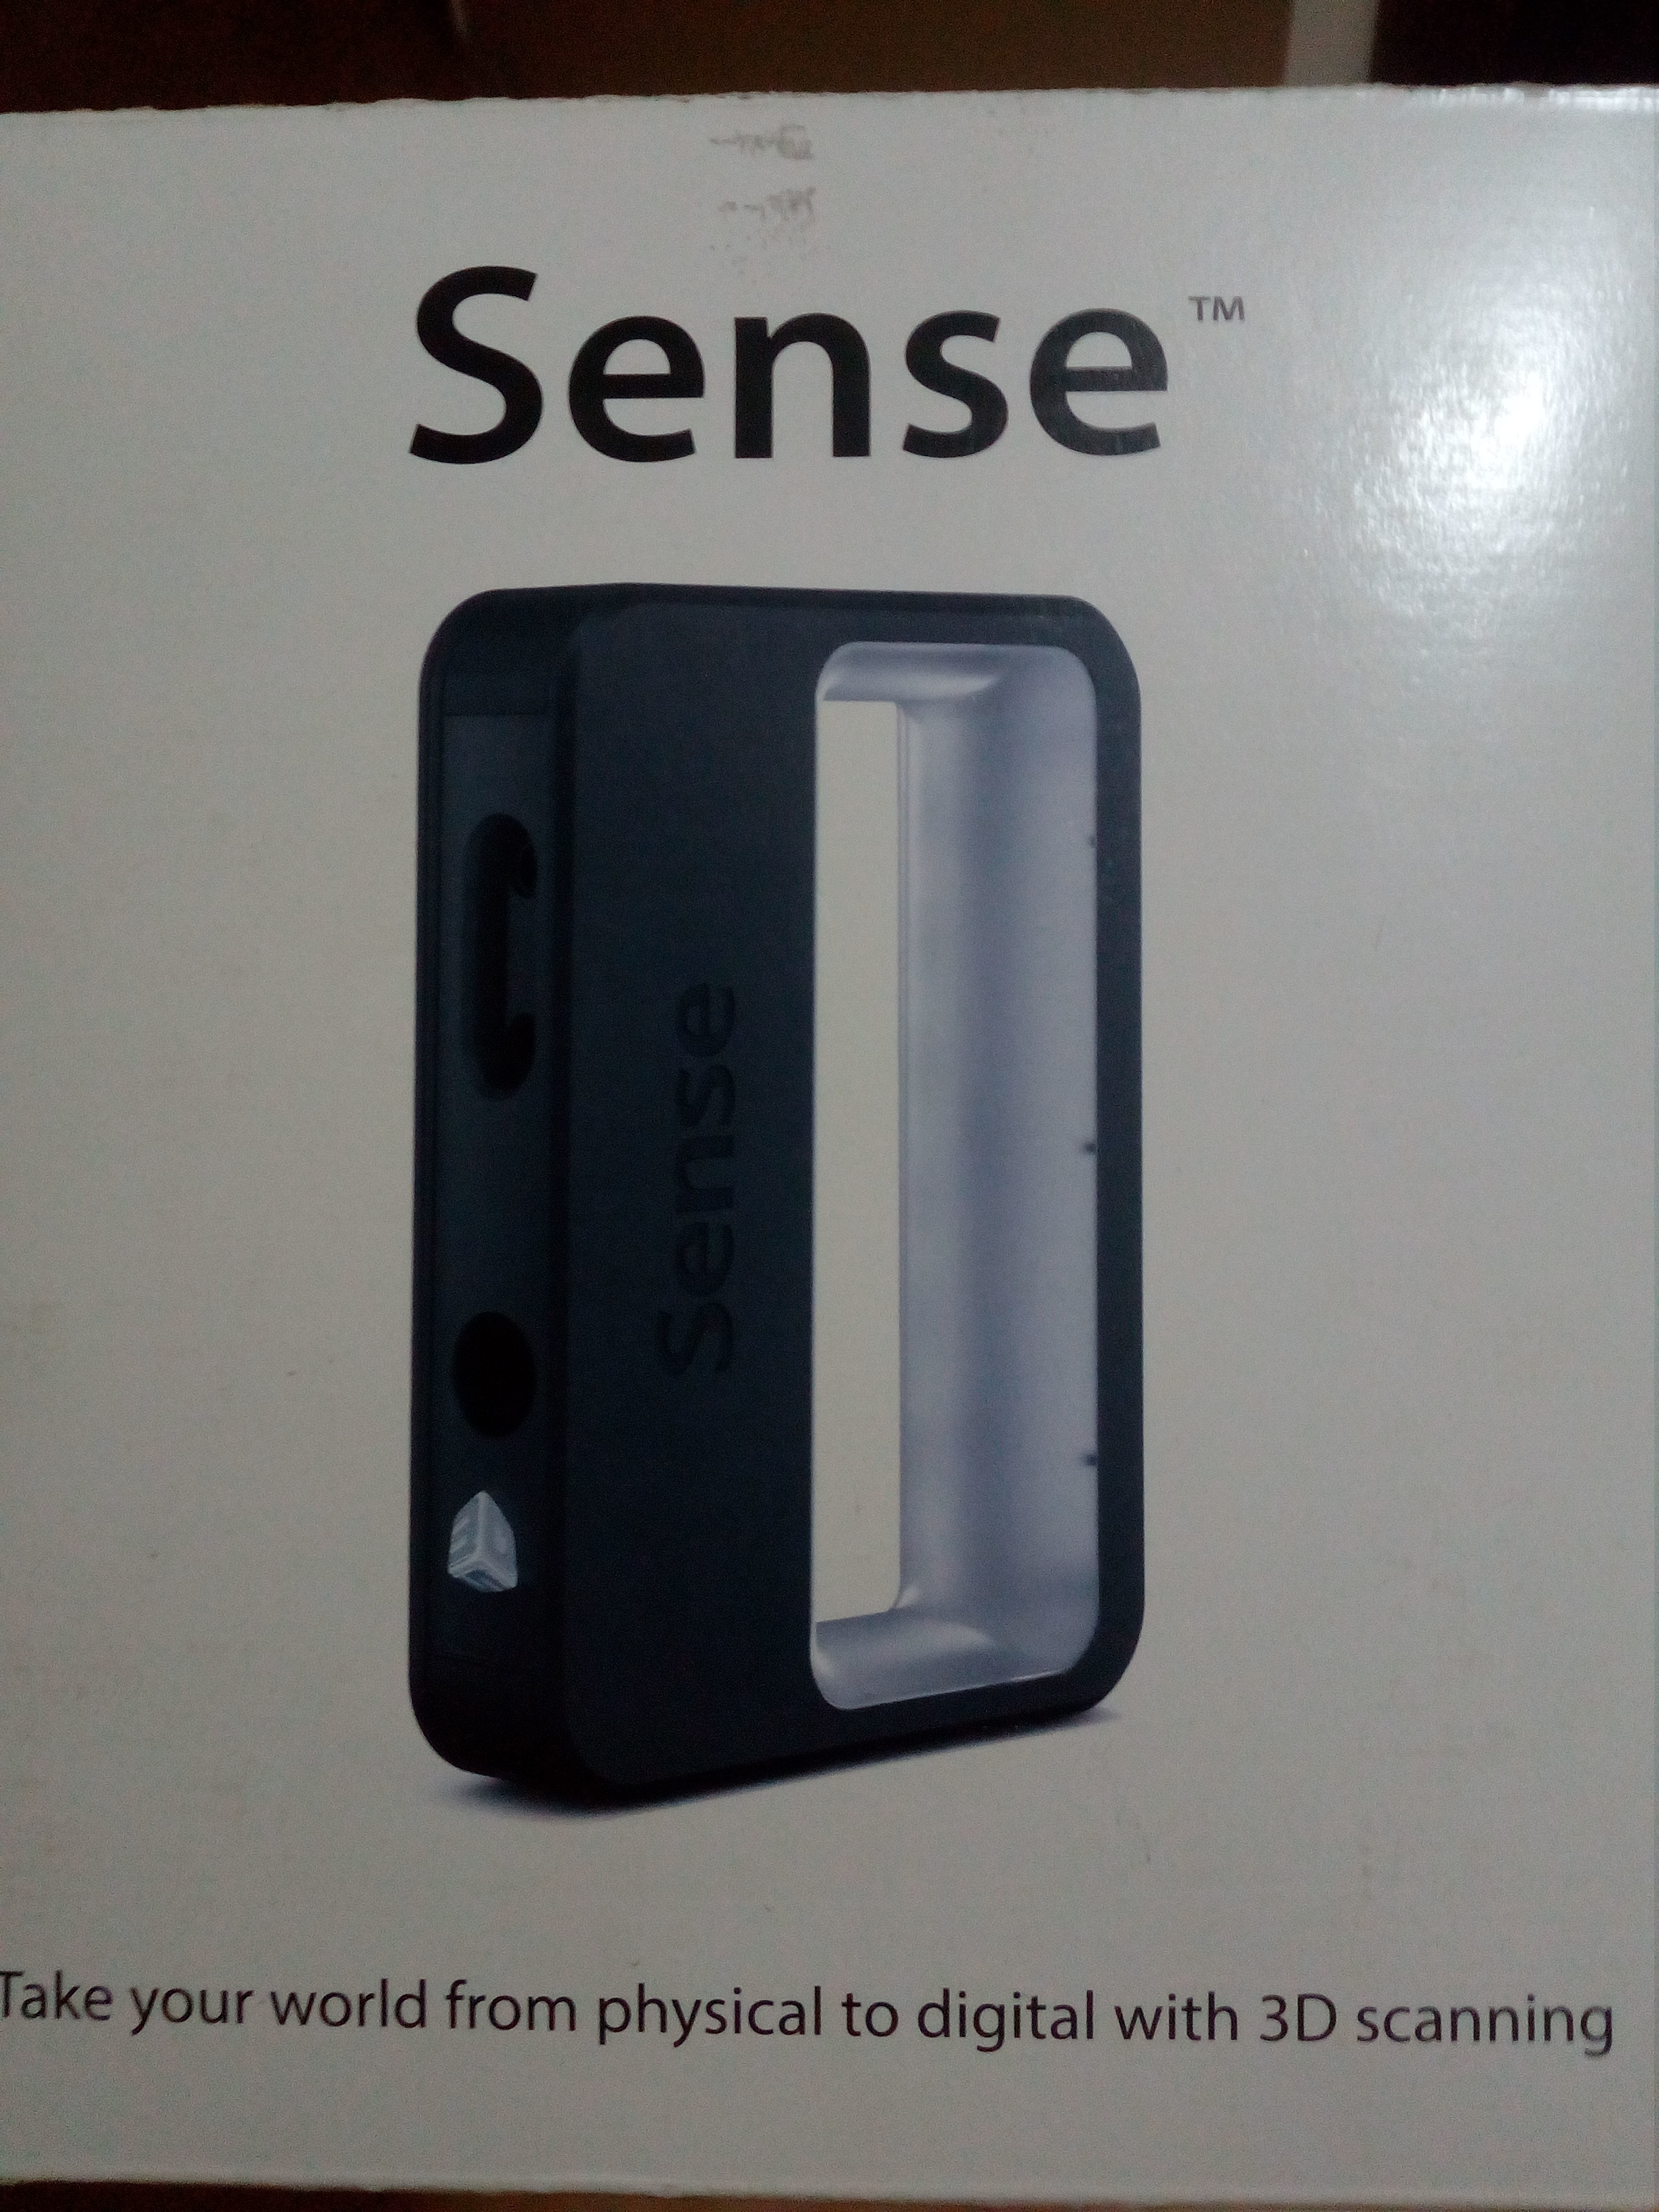
\includegraphics[width=0.75\linewidth]{figs/SenseFoto1.jpg}
	\source{
   	 O autor,
   	 2017.
   }
   \label{fig:fotoSense0}
\end{figure}

\begin{figure}[!h]
	\centering
	\caption{O Sense}
	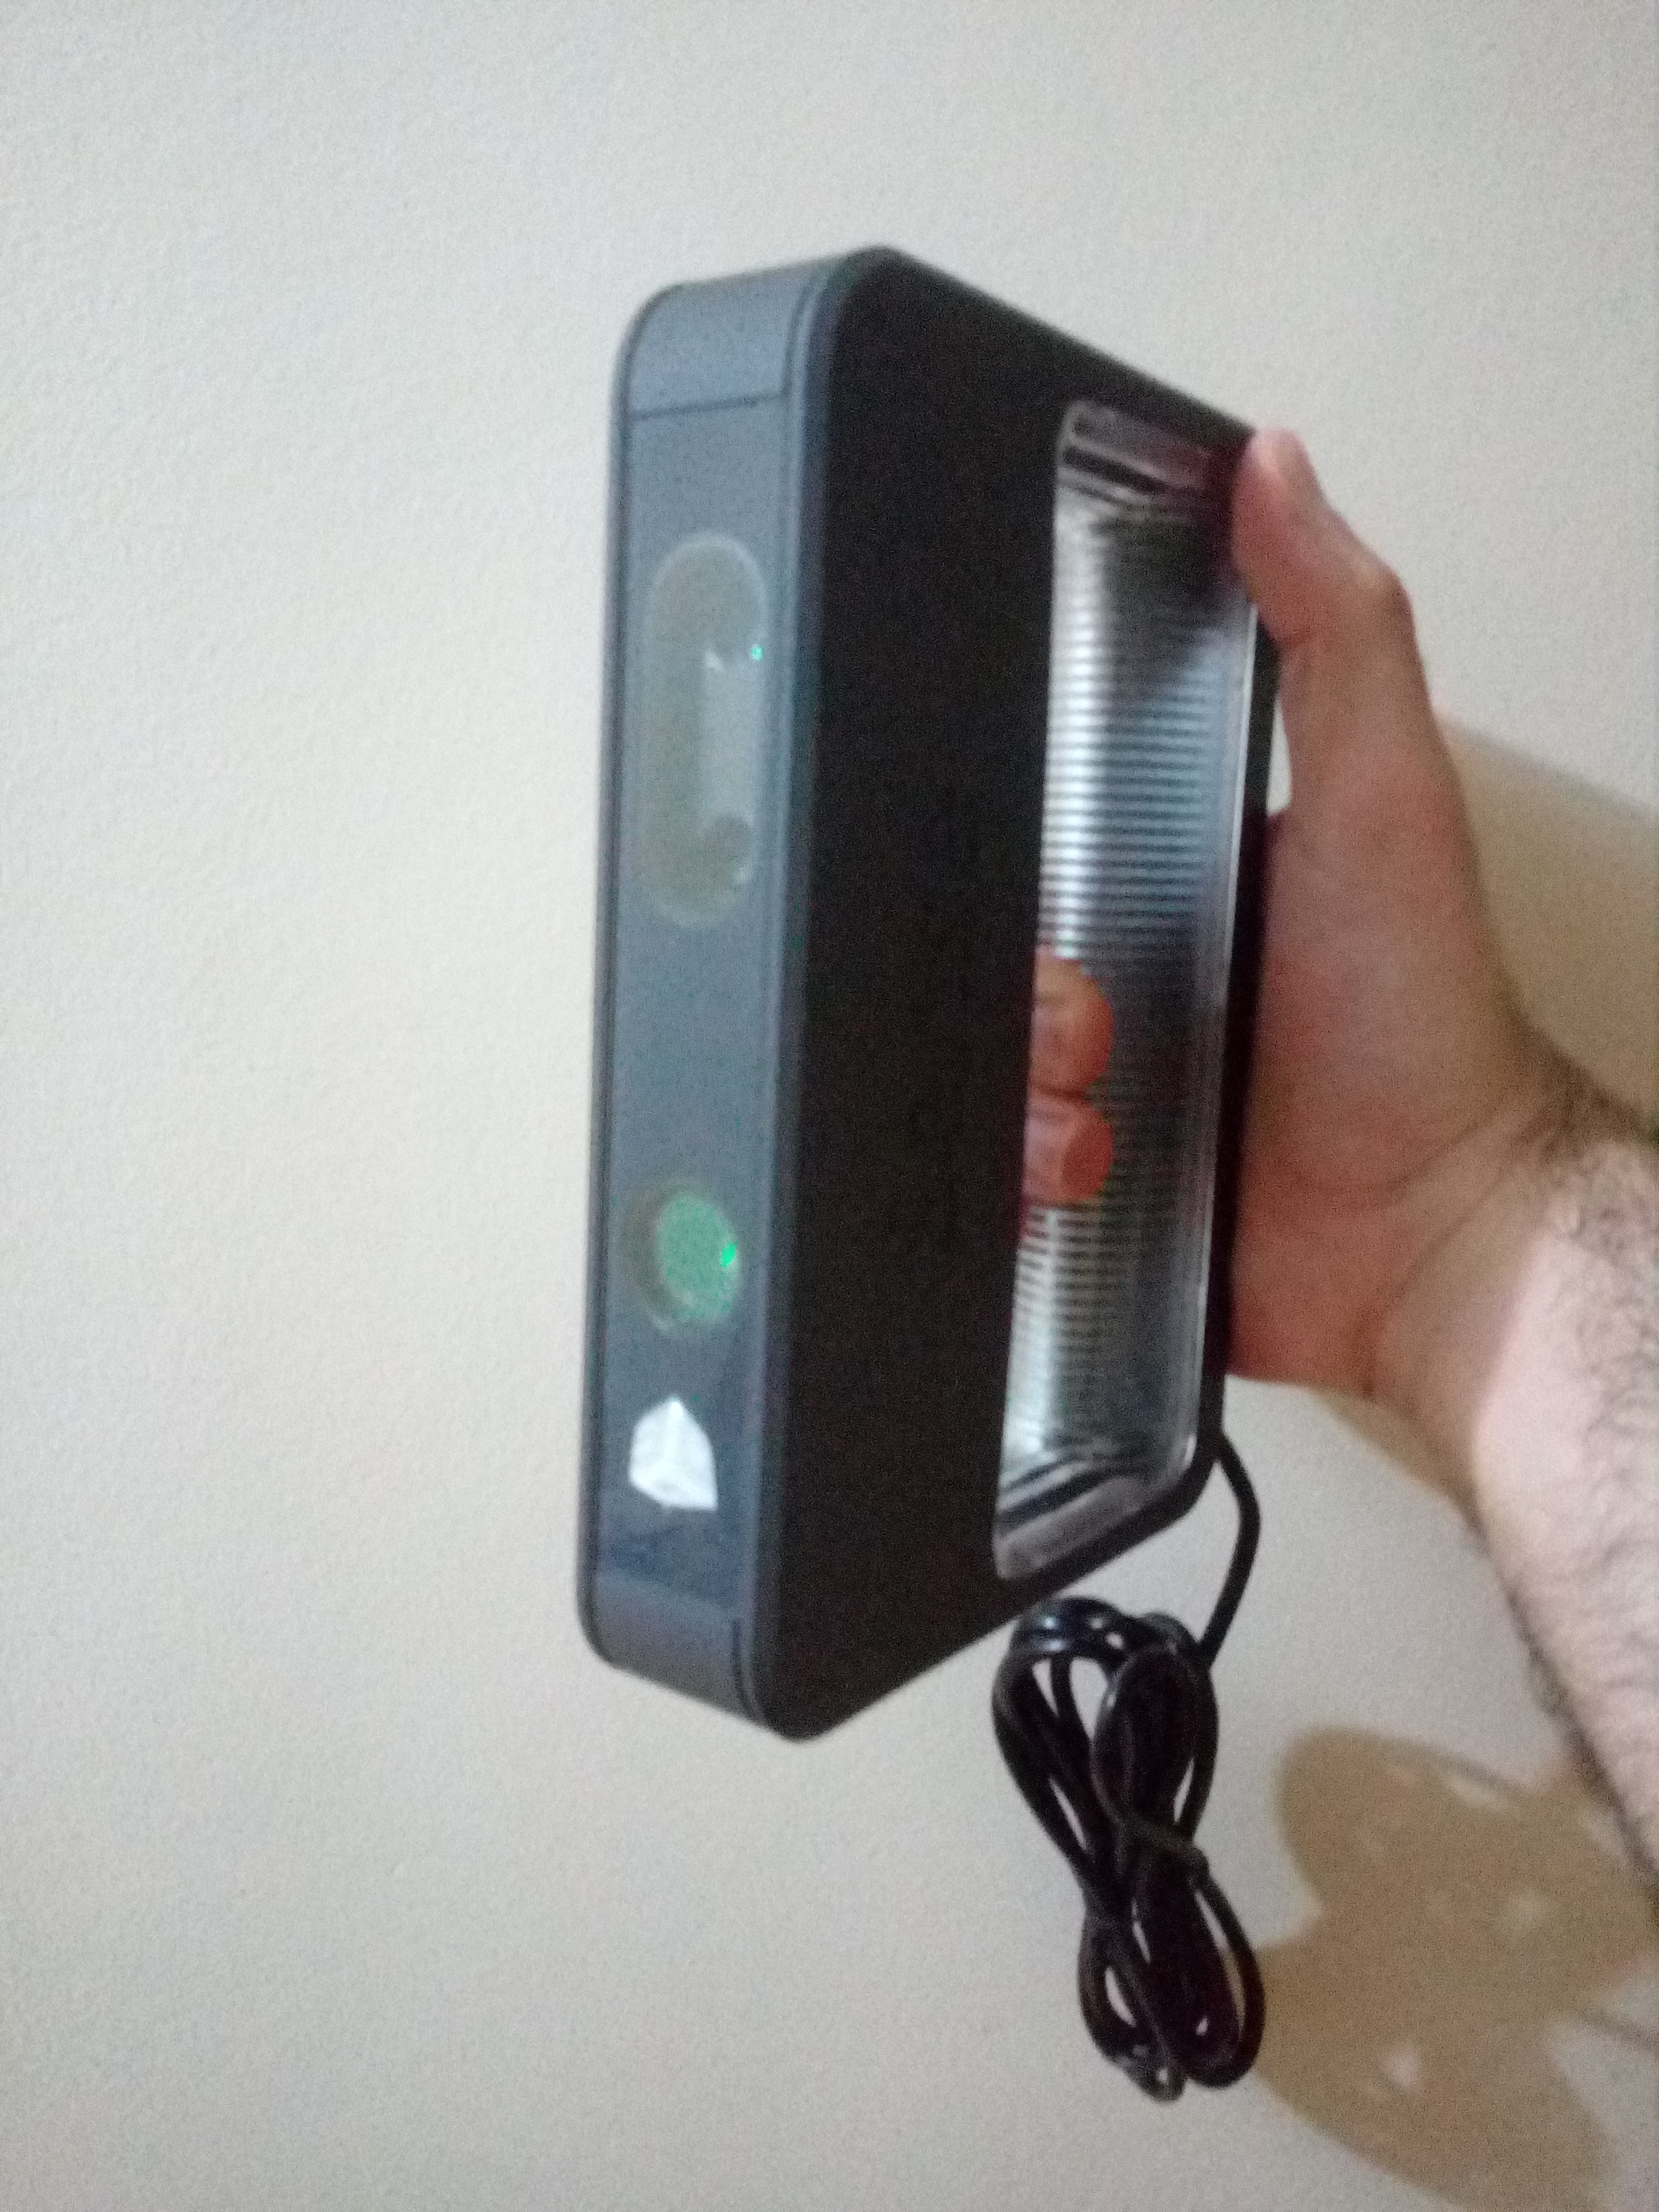
\includegraphics[width=1\linewidth]{figs/SenseFoto2.jpg}
	\source{
   	 O autor,
   	 2017.
   }
   \label{fig:fotoSense1}
\end{figure}

\newpage

Primeiramente devemos ativar e cadastrar o hardware no \emph{site} do proprietário e a partir disso, baixar o software.

O software do Sense é de fácil entendimento (figura~\ref{fig:sense0}), caso necessário, pode-se usar a tradução para o português e possui um \emph{link} para o guia do usuário onde é explicado todo o funcionamento da ferramenta e do seu software, bem como boas práticas para ter um bom resultado na reconstrução. O programa também conta com uma boa customização (como tamanho do objeto a ser escaneado, resolução, orientação, se desejamos reconstruir as cores, entre outros parâmetros). Além disso, ele faz uma rápida avaliação do computador e recomenda fazer a reconstrução a nível de GPU ou CPU, dependendo do resultado.

\begin{figure}[!h]
	\centering
	\caption{Tela inicial do Sense}
	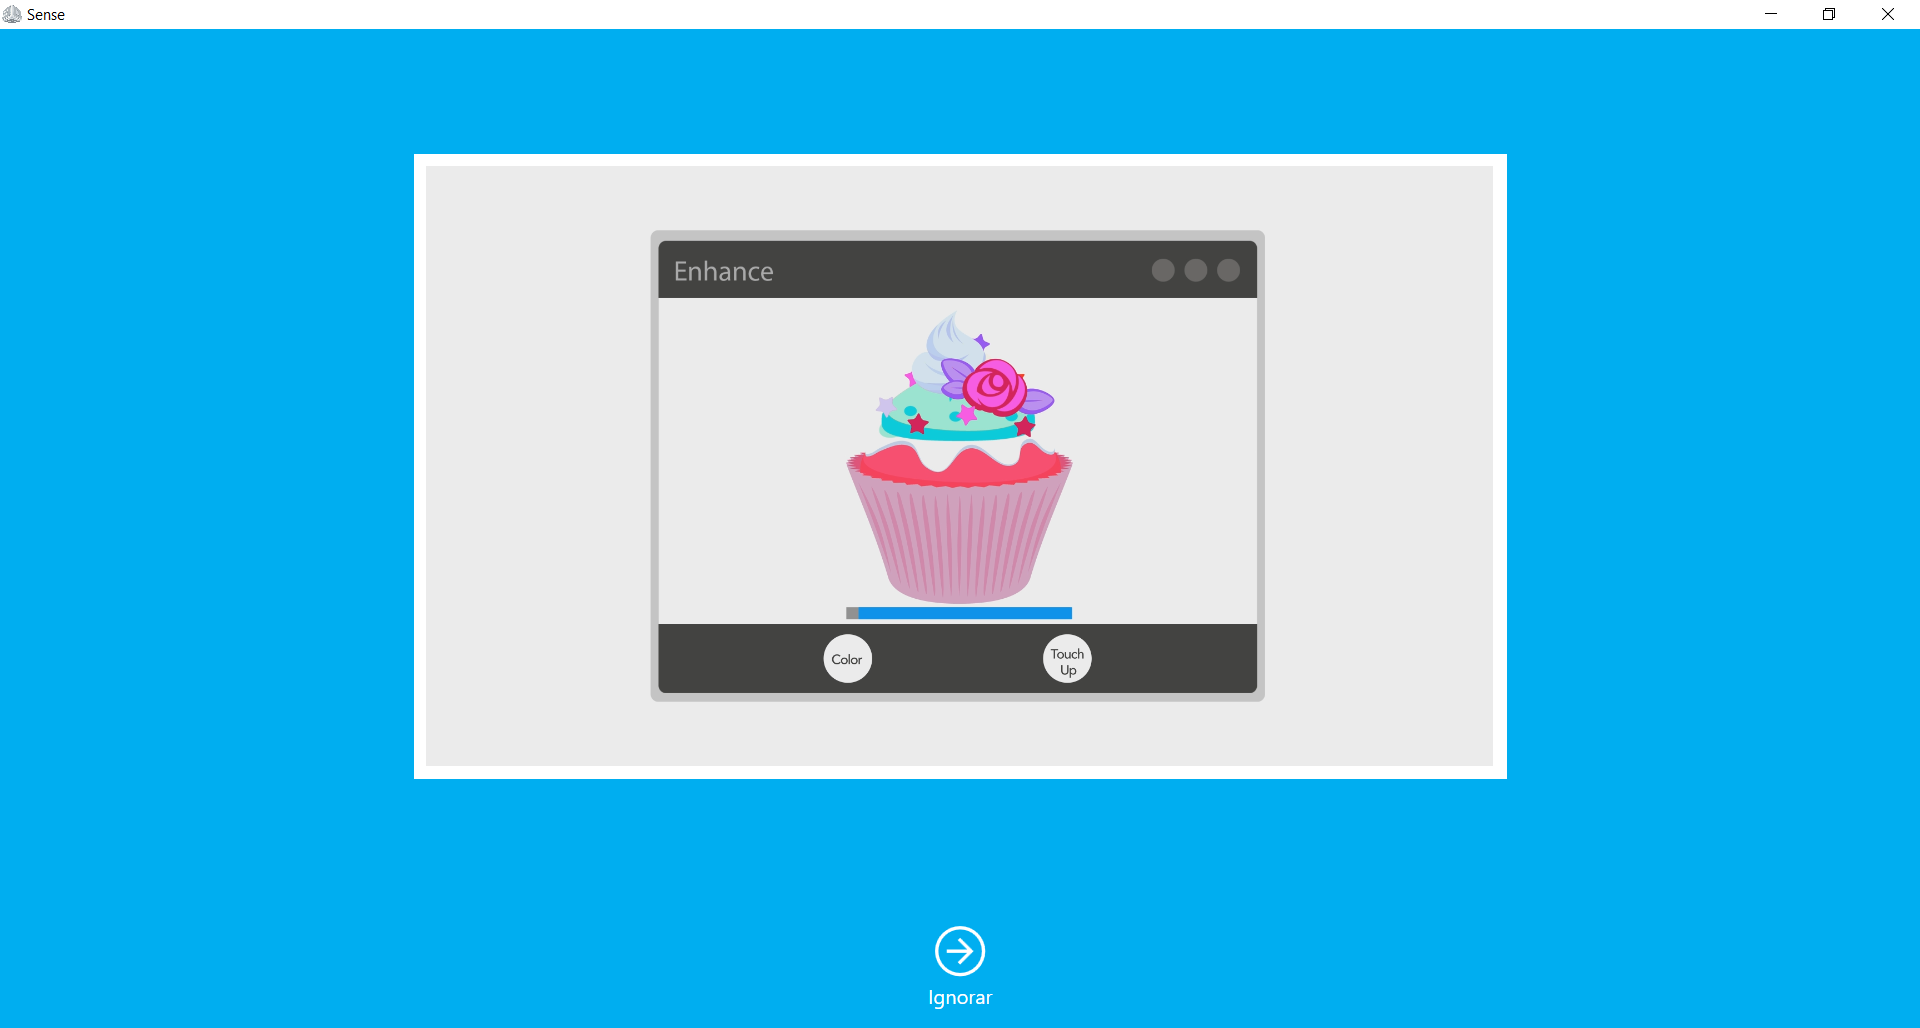
\includegraphics[width=1\linewidth]{figs/sense2v2.png}
	\note{Quando abrimos o Sense, temos à disposição um vídeo explicativo com algumas informações, como dicas para um bom escaneamento e sobre como manusear o software da maneira correta.}
		\source{
   	 O autor,
   	 2017.
   }\label{fig:sense0}
\end{figure} 

\newpage

\begin{figure}[!h]
	\centering
	\caption{Interface do Sense}		
	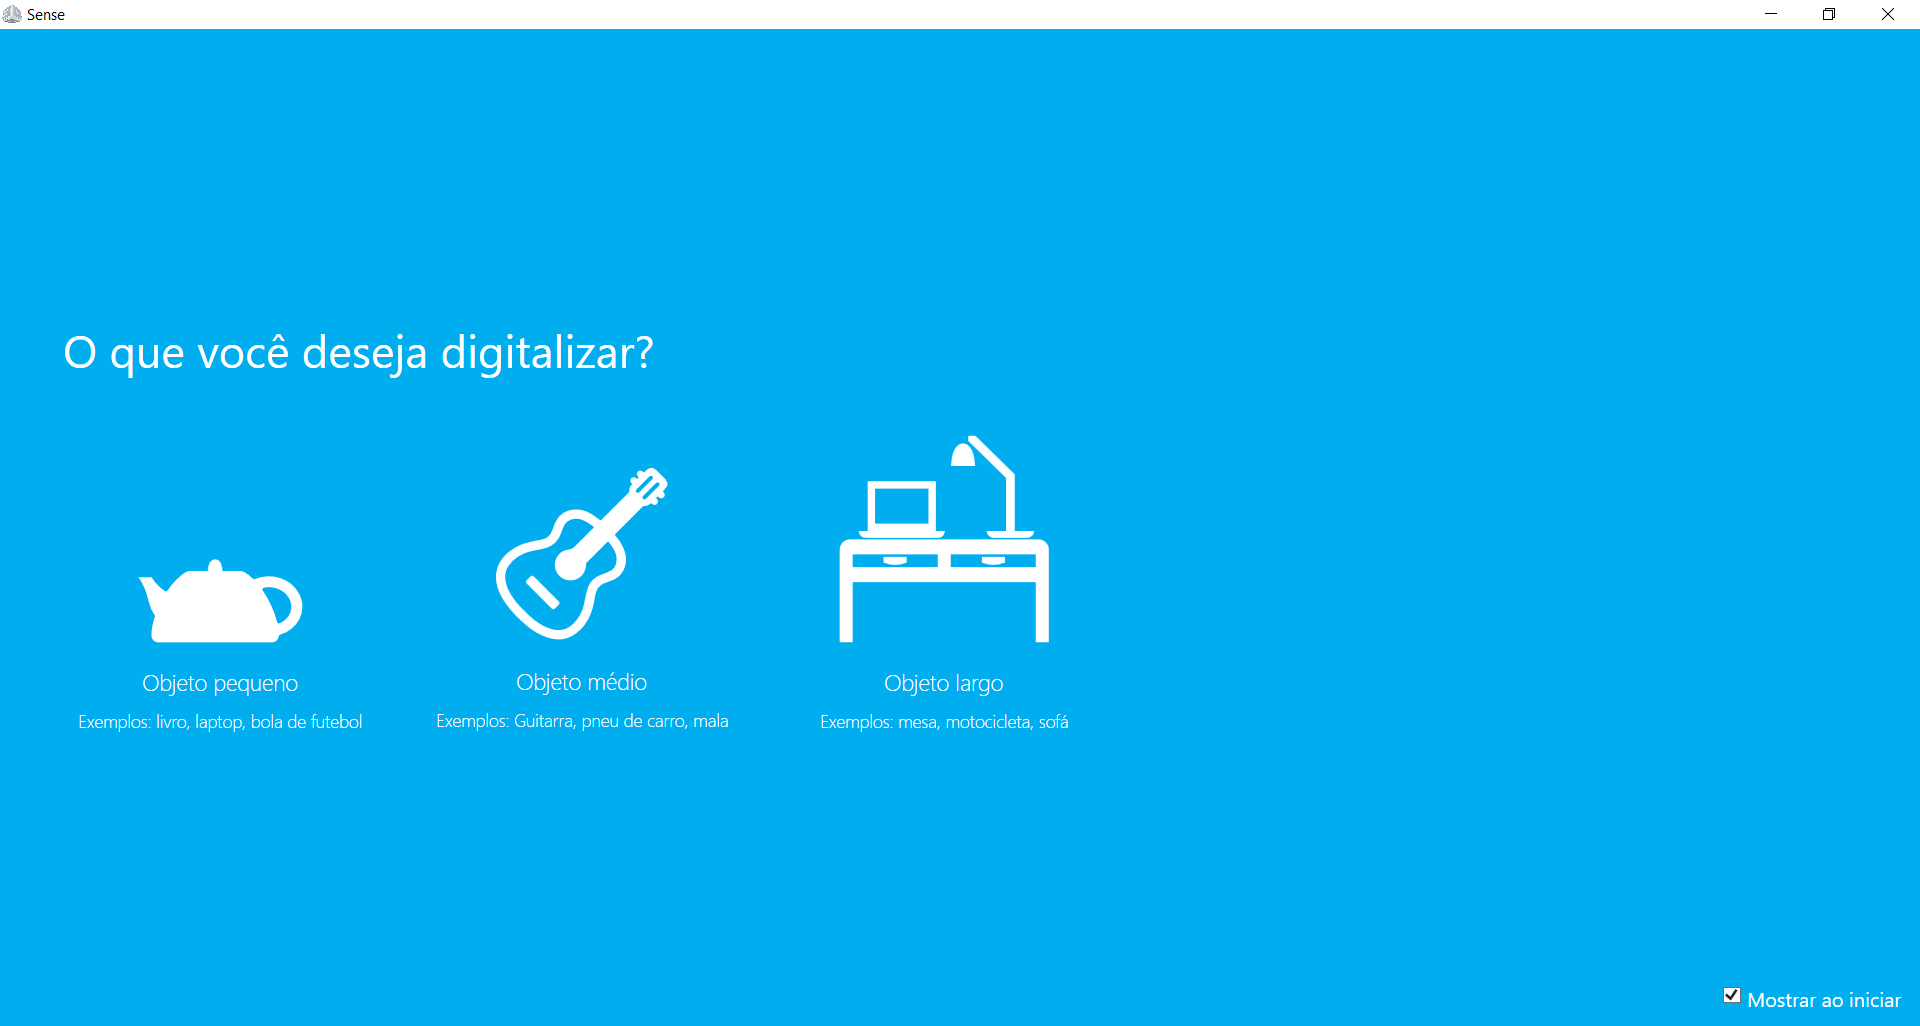
\includegraphics[width=0.8\linewidth]{figs/sense5v2.png}
	\note{Assim que passamos o vídeo introdutório, o software nos dá a opção de escanearmos uma pessoa ou um objeto. Onde ao escolhermos um objeto, podemos selecionar o tamanho do objeto a ser escaneado. Notamos que o próprio software indica que os menores objetos seriam um livro ou um laptop, por exemplo.}
	\source{
   	 O autor,
   	 2017.
   }\label{fig:sense1}
\end{figure} 

Para comparação com os softwares que foram descritos anteriormente, fizemos o escaneamento apenas do objeto em ambiente fechado. O Sense tem dificuldades de escaneamento em áreas abertas e pode não funcionar tão bem, como descrito no \emph{site} do proprietário~\cite{3DSystems}. 

Para a galinha, obtivemos os seguintes resultados.

\begin{figure}[!h]
	\centering
	\caption{Resultados do escaneamento com o Sense}
	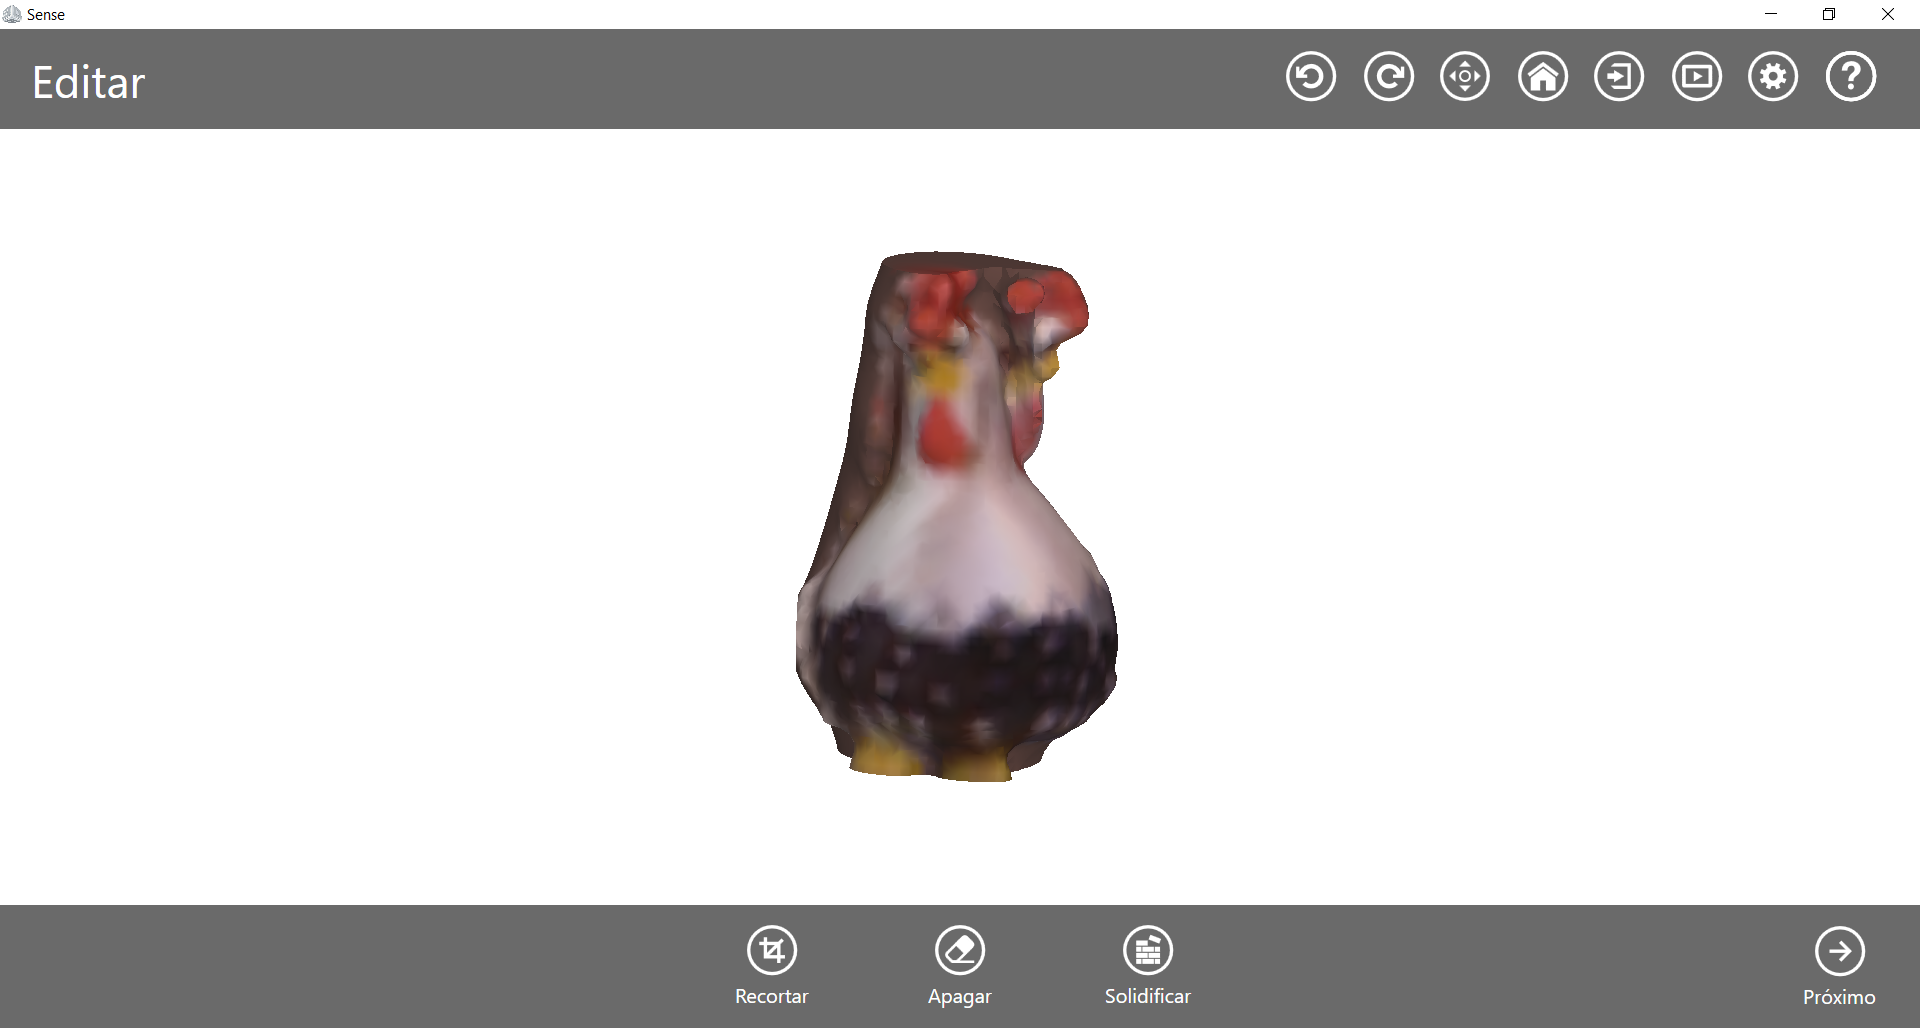
\includegraphics[width=0.8\linewidth]{figs/sense7v2.png}
%	\legend{Como resultado da digitalização, o Sense não se mostrou muito eficaz, pois gerou uma reconstrução com buracos e com poucas informações.}
		\source{
   	 O autor,
   	 2017.
   }\label{fig:sense3}
\end{figure} 

\newpage

\begin{figure}[!h]
	\centering
	\caption{Resultados do escaneamento com o Sense}
	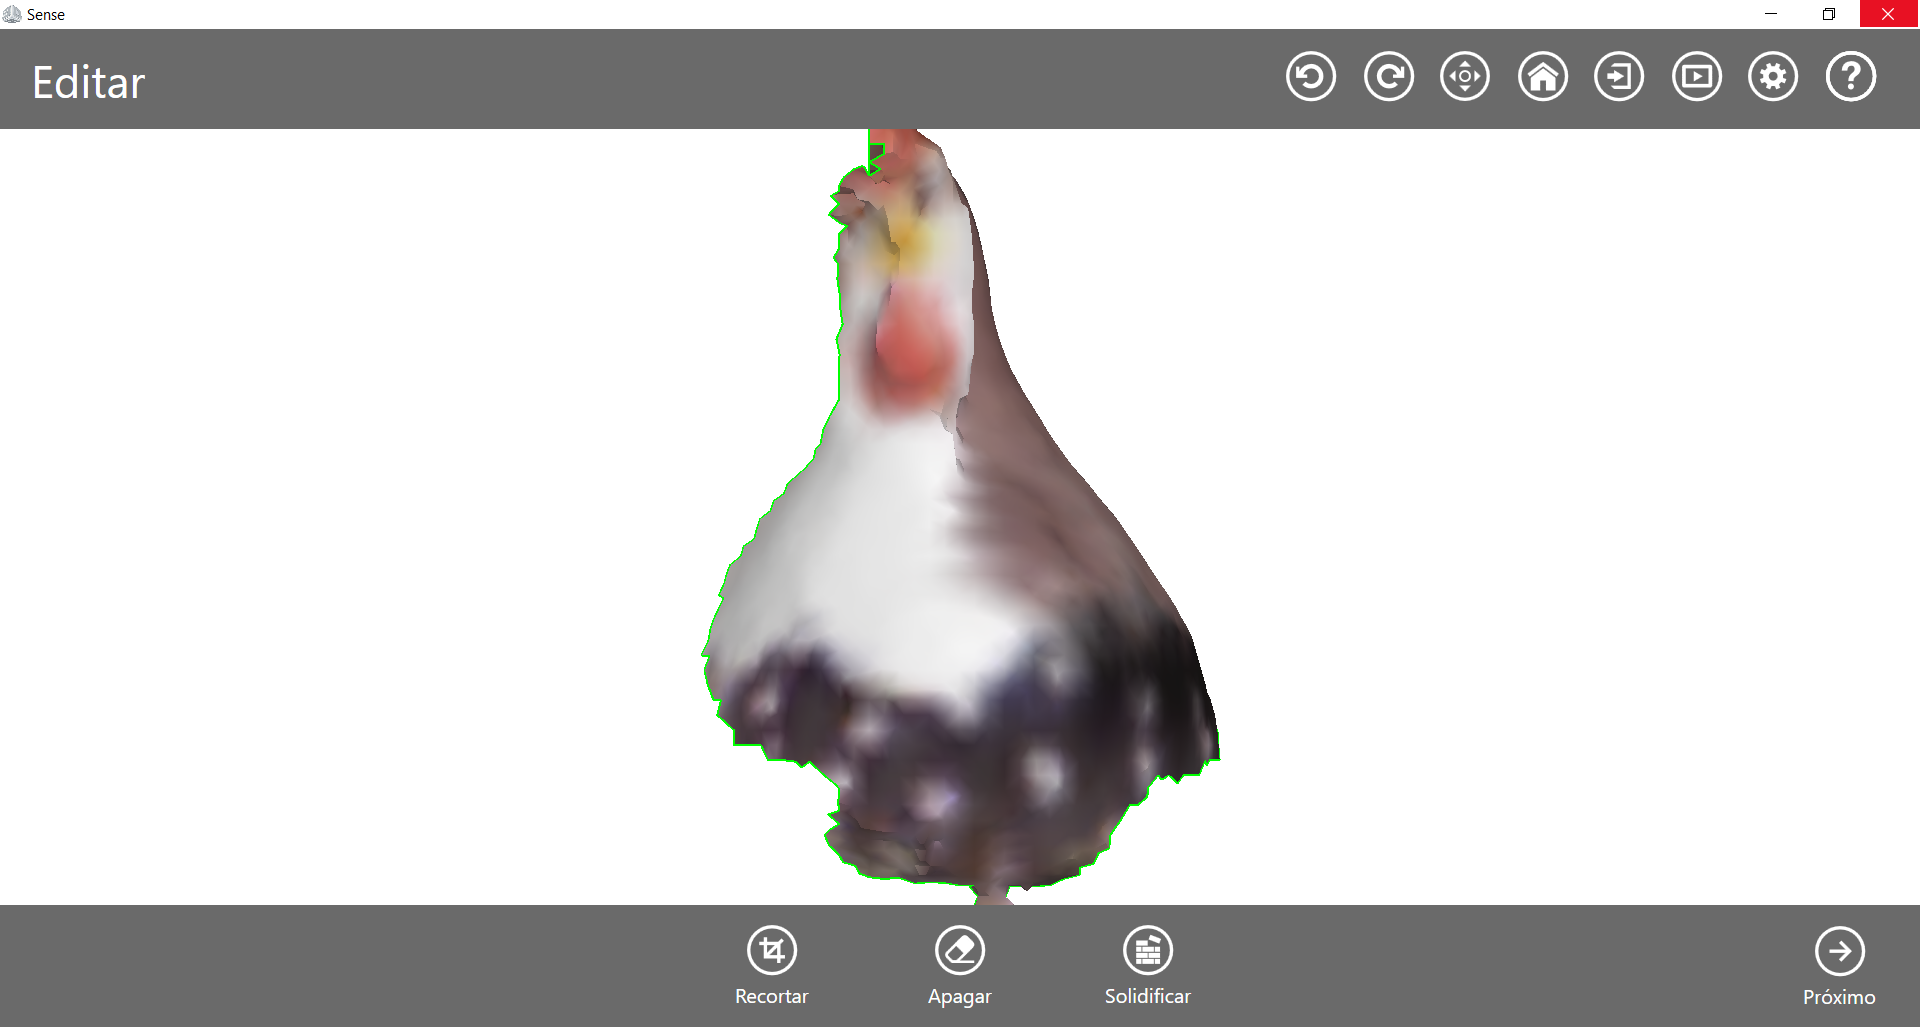
\includegraphics[width=0.9\linewidth]{figs/sense8v2.png}
	\note{Como resultado da digitalização, o Sense não se mostrou muito eficaz, pois gerou uma reconstrução com buracos e com poucas informações.}
		\source{
   	 O autor,
   	 2017.
   }\label{fig:sense3}
\end{figure} 


Os buracos e a falta de informações são decorrentes da perda de referência do objeto pelo software, solicitando ao usuário que volte ao ponto anterior para retomar a referência do objeto, o que geralmente é mais fácil recomeçar a digitalização do zero pois dificilmente o software consegue achar novamente a referência do objeto. 

Entrando em contato com o suporte do fabricante~\cite{3DSystems} fui notificado de que é necessário um computador com um processador Intel Core i5 ou superior e mesmo assim o software trava constantemente, o que torna o seu uso muito frustrante e que também colabora para a perda de referência do objeto.


%\begin{figure}[!h]
%	\centering
%	\caption{Resultado da reconstrução usando o Sense}
%	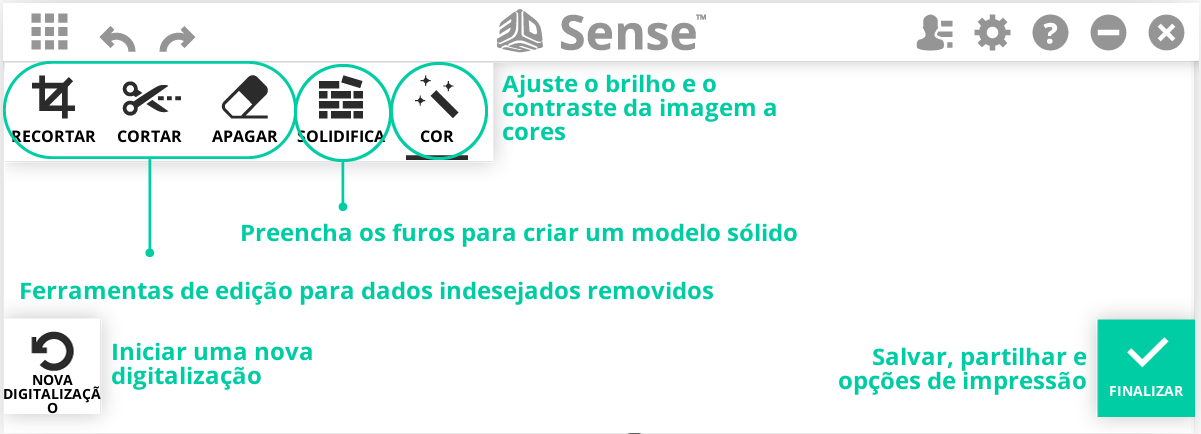
\includegraphics[width=1\linewidth]{figs/sense2.png}
%	\legend{Utilizando as práticas recomendadas para uma boa digitalização (em resumo, fazer uma varredura o objeto por inteiro, em diferentes ângulos), tivemos este resultado.}
%		\source{
%   	 O autor
%   	 (2017).
%   }\label{fig:reconSense1}
%\end{figure} 
%
%\begin{figure}[!h]
%	\centering
%	\caption{Resultado após ajustes de edição do modelo}
%	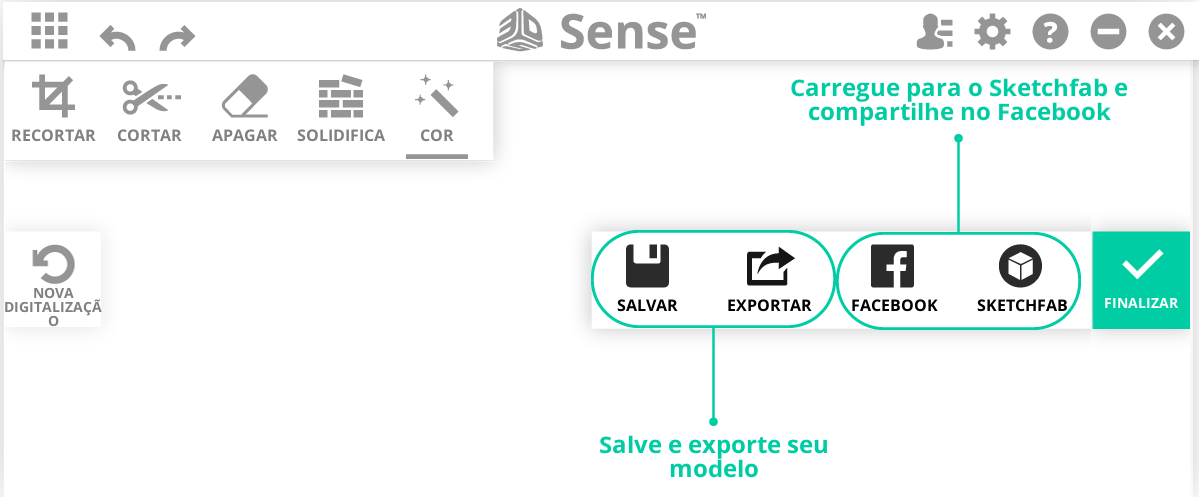
\includegraphics[width=1\linewidth]{figs/sense3.png}
%	\legend{Tratamos o modelo reconstruído preenchendo furos (provenientes da falta de informação daquele ponto).}
%		\source{
%   	 O autor
%   	 (2017).
%   }\label{fig:reconSense2}
%\end{figure} 
%
%\clearpage
%
%\begin{figure}[t!]
%	\centering
%	\caption{Resultado final usando o Sense}
%	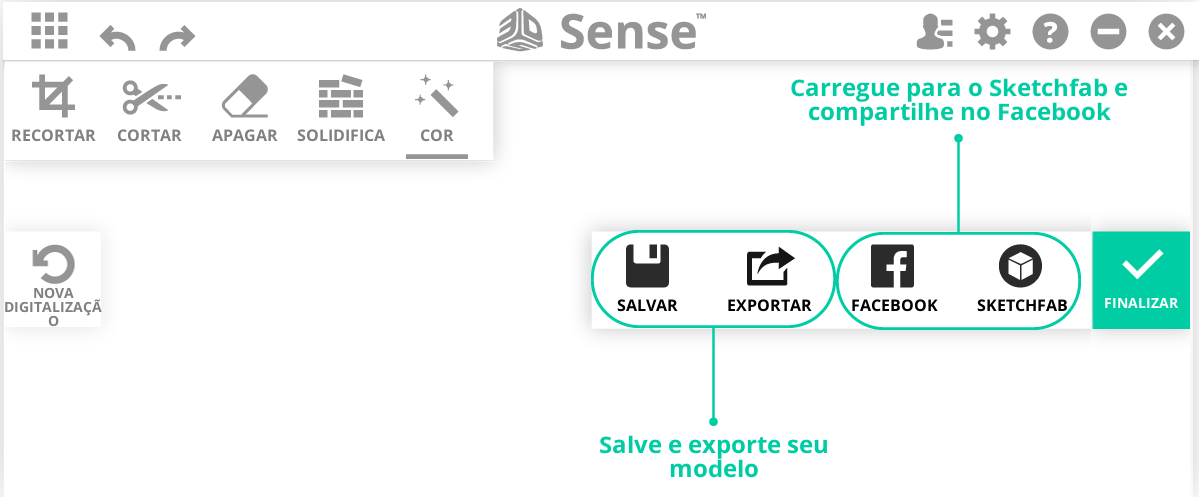
\includegraphics[width=1\linewidth]{figs/sense3.png}
%		\source{
%   	 O autor
%   	 (2017).
%   }\label{fig:reconSense3}
%\end{figure}

Não avaliamos o tempo de reconstrução, pois o Sense (assim como o Kinect) faz o escaneamento em tempo real.